
% Flexible plates
%\documentclass[reprint,amsmath,amssymb,aps,pre,longbibilography]{revtex4-1}
%\documentclass[reprint,amsmath,amssymb,aps,aip]{revtex4-1}

%\documentclass[twocolumn,aps,pre,amsmath,amssymb,floatfix,longbibilography]{revtex4-1}
\documentclass[aps,pre,twocolumn,aps,longbibliography]{revtex4-1}
\usepackage{amssymb}
\usepackage{amsmath}
\usepackage{graphicx}
%\usepackage{dcolumn}% Align table columns on decimal point
%\usepackage{subfigure}
%\usepackage{bm}% bold math
%\usepackage{setspace}
\usepackage{mathrsfs}
\usepackage{color}
\usepackage{ulem}
\newcommand{\volume}{{\ooalign{\hfil$V$\hfil\cr\kern0.08em--\hfil\cr}}}
\usepackage{lineno}
\linenumbers

%%%%%%%%%%%%%%%%%%%%%%%%%%%%%%%%


\begin{document}
	
	%\preprint{APS/123-QED}
	
	\title{Wall mounted flexible plates in a two-dimensional channel\\ trigger early flow instabilities}
	
	
	
	\author{Gaurav Singh$^1$}
	\author{Rajaram Lakkaraju$^1$}%
	\email{rajaram.lv@gmail.com}
	\affiliation{$^1$Computational Mechanics Group, Department of Mechanical Engineering,\\ Indian Institute of Technology Kharagpur, West Midnapore, Bengal, India-721302
	}
	\date{\today}
	
	\begin{abstract} 
		
		High level of mixing by passive means, is a desirable feature in microchannels for various applications, and use of flexible obstacles (or plates) is one of the prime choices in that regard. To get further insight, we have carried out two-dimensional numerical simulations for flow past one or two flexible plates anchored to a channel's opposite walls using fluid-structure interaction framework. On the inlet flow Reynolds number vs. the Strouhal number plane, we observed a sudden flow change from a laminar to a time-periodic vortex shedding state, when flexible plates are present in the channel. We found the critical Reynolds number as $Re_{cr}\approx 370$ when a single plate is anchored on the channel wall and $Re_{cr}\approx 290$ or even lower when two plates are anchored. With an increase in the inlet flow Reynolds number (up to 3200), we found vortices detach regularly at the plates' tips, which cause the flow to meander in the channel. In a two-plate anchored configuration, primary vortices generated at the first plate are constrained by the second plate, and result in an energetic secondary vortex generation in the downstream side. The overall flow features and the energy dissipation in the channel are mainly controlled by the separation gap between the plates. At high inlet flow Reynolds numbers ($\ge 1600$), the probability density function ($\mathcal{F}$) of the kinetic energy dissipation in a flexible plate configuration shows a stretched exponential shape in the form $\mathcal{F}(Z)\sim{\frac{1}{{\sqrt{Z}}}e^{-pZ^q}}$, where $Z$ is the normalized kinetic energy dissipation and the constants, $p=0.89$ and $q=0.86$. The observed increase in energy dissipation comes at the cost of an increase in pressure loss in the channel, and we found that the loss is inversely related to the plates' separation gap. From our simulations, we found that if high mixing levels are desired, then two flexible plates anchored to the channel walls is a better choice than a channel flow without obstacles or flow past a single plate. The two plate configuration with zero separation gap between the plates suits the best to achieve high mixing level.
		
		
		
	\end{abstract} 
	
	
	\maketitle
	
	
	\section{Introduction}
	Fluid flow over elastic objects involves hydrodynamic and structural instabilities that manifest in the form of a wide range of flow scale generation, self-induced structural oscillations, and acoustic noise~\cite{Balachandar1999, Zhang2000, Hall2001, Mahadevan2004, Vandenberghe2004, Shelley2011}. Few examples where the fluid-structure interactions (FSI) have significance are human phonation~\citep{Mittal2013}, blood flow through arteries and veins~\citep{Manz2002,Verzicco2009}, bio micro-flow devices~\cite{Khatvakar2007}, wing flutter~\cite{Taneda1968}, and wind farms~\cite{Klienstreuer2009}. Flow past a flexible structure can trigger various forms of instabilities when an imbalance takes place between the de-stabilizing hydrodynamic forces and the stabilizing elastic restoring forces~\citep{Taneda1968, Zhang2000, Watanabe2002, Eloy2008, ZhuPeskin2002, Alben2008}. Usually, the transport rates are high when an instability unveils in the flow. The increase of transport rates in a channel is highly beneficial in applications like micro-total analysis~\citep{Manz2002}, where quick and thorough mixing is of utter importance. In some other applications also, like heat exchangers or chemical reactors, increased mixing level is highly desired. The mixing can be prompted and enhanced by placing obstacles (passive methods) or actuators with an external power source (active methods) in the channels. The passive methods are simple and are relatively easy to integrate with various systems. These do not require any additional power units and mainly depend on the flow inertia. Some such passive mixing designs include repeated asymmetric grooves, rigid laminations, s-shaped serpentine channels and others~\citep{Whitesides2002, Nguyen2005, Squires2005, Kashid2011, Kang2015}. By using flexible plates instead of rigid laminations in the channel~\cite{LambertRangel2010, Khatvakar2007}, a significant increase in transport rate is observed. In specific devices such as bio-pumps, micro heat exchangers and cell sensors, the anchored flexible plates on the channel walls undergo self-sustained oscillations and act as actuators, and hence, increase the transport rates.
	
	Flow through microchannel devices is usually considered as planar due to insignificant flow variations in the depth direction~\cite{Khatvakar2007, LambertRangel2010, Stone2001}. The channel length to height ratio ranges from six to twelve, and the flow evolves throughout the channel length~\cite{Beebe2010, Whitesides2006, Liu2010}. Any theoretical framework to find the transport rates in such channels with developing flow features is difficult to explore. Experiments are promising for the pressure loss measurements in a microchannel, but the main challenge lies in capturing the erratic flow and plate motions. So, numerical simulations become the best choice to explore such intricate details.
	
	Inspired by the research works on microchannel flow \cite{Khatvakar2007, LambertRangel2010, Gleeson2005, Pathak2012, Kim2010, Stone2001, Stone2004}, we have carried out two-dimensional numerical simulations to understand flow past one or two flexible plates, each of half the channel height, anchored to the channel walls in a staggered fashion (as shown in figure \ref{fig:schematic}). The proposed staggered design is influenced by the works of~\cite{Asgar2007}, in which an excellent mixing performance is observed for such arrangement of obstacles in a microchannel. The separation gap between the plate 1 and the plate 2 (denoted by $d$) is decreased systematically to analyze the local blockage created by the plates and its effect on the flow in the downstream side. We have also varied the inlet flow Reynolds number $Re$, to investigate the resulting flow and the plate motions. We have enforced strong coupling between the fluid and the structure (or the anchored plates) in our simulations, such that each can affect one another. In the subsequent sections, we show that, by using the flexible plates in the channel, one can change the flow from the laminar to a chaotic regime and can observe an increase in the energy dissipation rates.
	
	
	
	The article is organized as follows: In section II, we have described the mathematical model and the computational procedures to solve the fluid-structure interaction problem. In section III and IV, detailed study on the plate deflections and the flow fields are presented. In section V, the tip generated vortices, and their dynamics are explained. In section VI, the energy dissipation and the pressure loss in the channel are discussed. Finally, we have summarised the results in the end.
	
	
	\begin{figure}
		\begin{minipage}[c]{1\linewidth}
			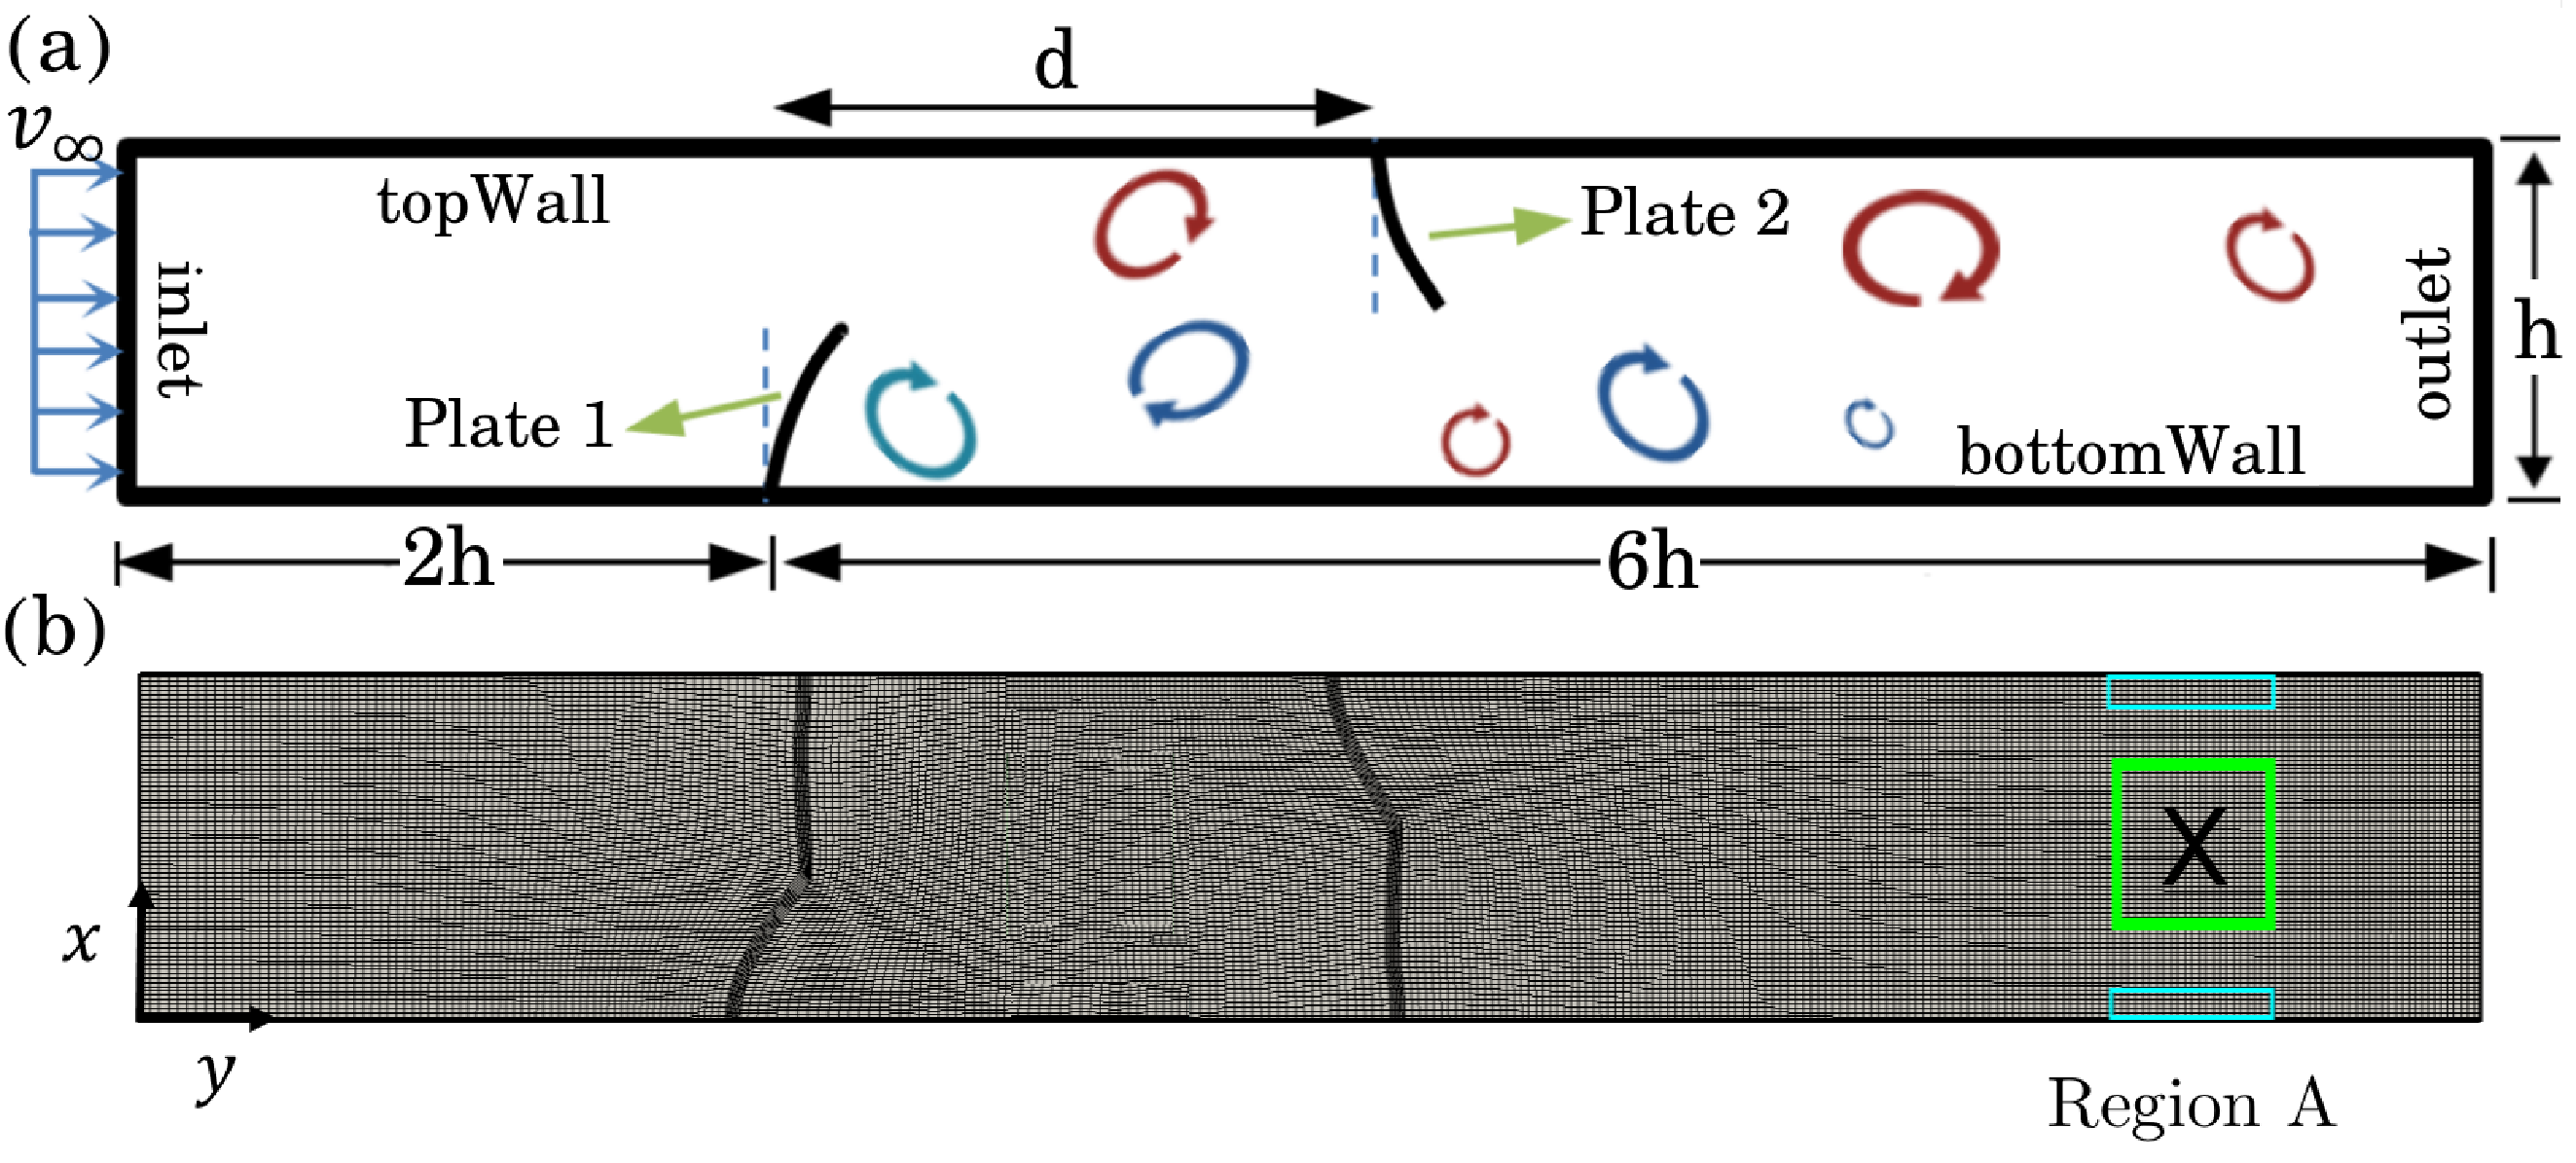
\includegraphics[width=1\linewidth]{Fig01.pdf} 
		\end{minipage} 
		\caption{(a) Schematic of a two-dimensional flow past flexible plates. A uniform flow enters at the inlet, passes over the plates and leaves from the outlet. The channel is $8h$ in length and $h$ in height. The plates are of height $l= 0.5h$ each. (b) A typical computational mesh used in our simulations. Dissipation statistics and frequency measurements are taken in Region A. Core zone in big rectangles and boundary layers in small rectangles.
		}
		\label{fig:schematic}
	\end{figure}
	
	\section{Mathematical formulation and computational procedure}
	
	In our work, we have considered a strong coupling between the fluid and the structure (or the plate) such that each of these can influence the other. The governing equations are formulated by using the Arbitrary Lagrangian Eulerian (ALE) framework, in which the change in volume of each control element between two adjacent time steps is always equal to the volume swept by the mesh, see more details in~\cite{Nguyen2010, Slone2002, CampbellPaterson2011}. The flow is assumed to be incompressible and Newtonian, and the mass and momentum equations for the fluid are given as,
	\begin{eqnarray}
	\nabla\cdot\left[(\mathbf{v}_f-\mathbf{v}_m)\right] &=& 0, \\
	\rho_f\left[{\partial\mathbf{v}_f\over\partial t}+\left[(\mathbf{v}_f-\mathbf{v}_m)\cdot\mathbf{\nabla}\right]\mathbf{v}_f\right] &=& \mathbf{\nabla}\cdot\mathbf{\boldsymbol{\sigma}}_f,
	\end{eqnarray}
	where $\rho_f$ is the fluid density, $\mathbf{v}_f=(v_x,v_y)$ is the flow velocity, $\mathbf{v_m}$ is the velocity of the mesh motion and $\boldsymbol{\sigma}_f$ is the total stress tensor. The operator ${\partial\over\partial t}$ is the partial derivative with time, and $\mathbf{\nabla}\equiv ({\partial\over\partial x},{\partial\over\partial y})$ is the spatial gradient computed on the $x$-$y$ plane. Divergence of the stress tensor for the incompressible and Newtonian fluid can be written as $\nabla\cdot\boldsymbol{\sigma}_f=-\mathbf{\nabla}P+\mu_f\mathbf{\nabla}^2\mathbf{v}_f$. Here, $P$ is the dynamic pressure, $\nabla^2$ is the laplacian operator, and $\mu_f$ is the fluid dynamic viscosity. 
	
	
	
	The plates' motion (or the displacement, $\mathbf{u}_s$), is computed on the Arbitrary Lagrangian framework on which the mesh velocity ($\mathbf{v}_m$) equals the material velocity, i.e., $\mathbf{v}_m\equiv {\partial\mathbf{u}_s\over\partial t}$. The Eulerian mesh (for the fluid) implementation follows $\mathbf{v}_m=0$, and for the Lagrangian mesh, it follows $\mathbf{v}_m=\mathbf{v}_f$. The suffixes $_f$, $_s$ and $_m$ correspond to fluid, solid and mesh, respectively. The momentum conservation equation for the flexible plate is given by,
	\begin{eqnarray}
	\rho_s{\partial^2\mathbf{u}_s\over\partial t^2} &=& \mathbf{\nabla}\cdot\mathbf{\boldsymbol{\sigma}}_s,
	\end{eqnarray}
	where $\rho_s$ is the plate density (which is assumed constant in our work), and $\mathbf{\boldsymbol{\sigma}}_s$ is the Cauchy stress tensor. We assumed a linear elastic material for the plate, for which the strain rate is defined in terms of the Lagrangian-Green's tensor, $\boldsymbol{\varepsilon}_s={1\over2}[(\mathbf{\nabla}\mathbf{u}_s+\mathbf{\nabla}\mathbf{u}_s^T)+(\mathbf{\nabla}\mathbf{u}_s - \mathbf{\nabla}\mathbf{u}_s^T)]$. Both the stress and the strain tensors are related as $\boldsymbol{\sigma}_s=2\mu_s \boldsymbol{\varepsilon}_s+\lambda( \mathbf{\nabla}\cdot\mathbf{u}_s)\mathcal{I}$. Here, $\mu_s=\mathcal{E}/[2(1+\kappa)]$ and $\lambda=\kappa \mathcal{E}/[(1+\kappa)(1-2\kappa)]$ are the Lame's constants, $\kappa$ is the Poisson's ratio, $\mathcal{E}$ is the Young's modulus, and $\mathcal{I}$ is the identity tensor of rank two. The superscript $^T$ denotes the transpose of a given tensor. The flow stress information and the structural displacement communicate with each other across the interface. We have strictly posed the no-slip condition on the channel walls and on the fluid-plate interface. Mathematically, these conditions correspond to $\boldsymbol{\sigma}_s\cdot\mathbf{n}=\boldsymbol{\sigma}_f\cdot\mathbf{n}$, and $\mathbf{v}_m={\partial\mathbf{u}_s\over\partial t}$, where $\mathbf{n}$ is the normal vector to the wall-fluid interface, see more details in~\cite{CasadeiHalleux1995, Casadei2001}. We have used the Laplace operator approach to compute the fluid mesh motion by solving $\mathbf{\nabla}\cdot(\gamma\mathbf{\nabla}\mathbf{v}_f)=0$, as mentioned in~\cite{JasakTukovik2006}. Here, $\gamma$ is a variable diffusion coefficient which is inversely proportional to the distance from the moving boundary. At the channel inlet, a uniform velocity ($v_{\infty}$) and a zero pressure gradient are applied, whereas, at the outlet, we maintained a zero-velocity gradient and a fixed (zero) pressure.
	\begin{figure}
		\begin{minipage}[c]{1\linewidth}
			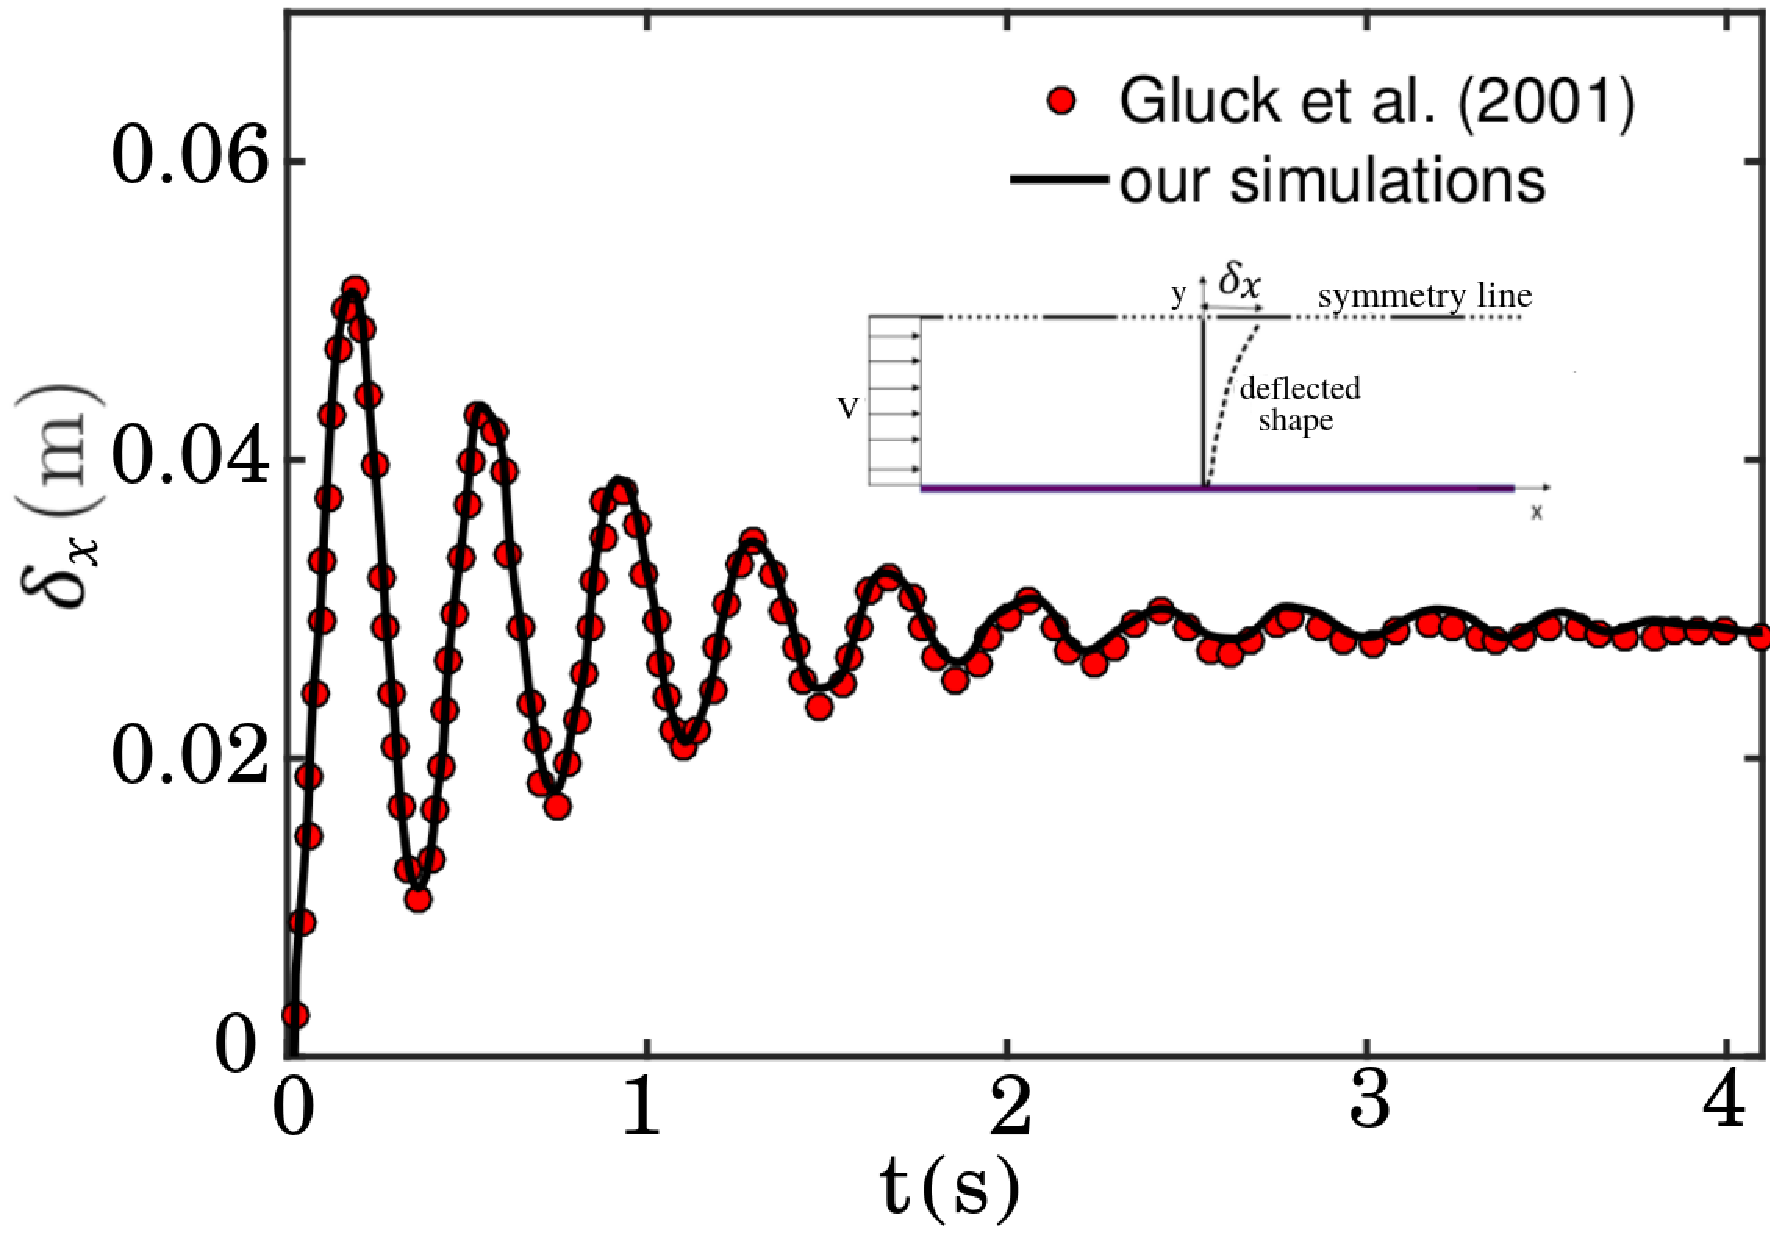
\includegraphics[width=1\linewidth]{Fig02.pdf} 
		\end{minipage} 
		\caption{Validation of our results with~\cite{Gluck2001}. Inset shows schematic of the problem considered.}
		\label{validation1}
	\end{figure}
	
	We have used finite volume method in which the temporal discretization is done using a second-order accurate Euler-implicit scheme, and the spatial discretization of the convection and diffusion terms by the central differencing with Gaussian integration. The Courant number, which is based on the local velocity (magnitude), the time-step of integration and the length of the computational cell, is always kept below 0.2 in our work. The mentioned governing equations are solved as follows, (1) at any given instant, the intermediate flow velocity is computed for an assumed pressure field, then (2) a new pressure field is calculated from the pressure-Poisson equation. This is followed by (3) calculating a correct velocity field which satisfies the divergence-free condition at the next time-step. Based on the resulting stress from the fluid domain, we have computed the solid displacements. Finally, the required mesh-displacements for the fluid mesh are computed by using the Aitken dynamic relaxation along with the Laplace operator approach. A detailed computational algorithm can be found in Refs.~\cite{Hrvoje2007, CampbellPaterson2011}.
	
	Foremostly, we performed a validation study to establish confidence in the reported results. We considered a test case where a plate oscillates in a fluid flow, as shown in figure 12 of~\cite{Gluck2001}. In figure~\ref{validation1}, we have computed tip deflection vs. time and compared with the results as mentioned in section 3.1.2 of~\cite{Gluck2001}, and an excellent agreement is found with our simulations.
	
	
	
	
	
	After the validation study, we proceed further to understand flow past flexible plates in a channel of height $h$ and length $8h~(=L)$ as shown in figure~\ref{fig:schematic}. The anchored plates are of height $l=0.5h$, and thickness $w=0.01h$. The chosen geometry is nearly similar to~\cite{Jin2018}, where flow past a single flexible plate anchored on a channel wall is studied. In our work, the characteristic velocity is $v_\infty$, and the characteristic length is based on the flow gap between the wall and the anchored plate, i.e., $(h-l)=0.5h~(=l)$. The dimensionless parameters are the Reynolds number $Re=v_{\infty}l/\nu$, the density ratio $\rho_s/\rho_f$, and the ratio of fluid inertia to elastic restoring force $\beta=\rho_f v_{\infty}^2 l^3 b/(\mathcal{E}I)$, where $\nu$~($=\mu_f/\rho_f$) is the kinematic viscosity of the fluid, $I=bw^3/12$ is the plates' moment of inertia and $b$ is the plate depth (normal to x-y plane)~\cite{Bhageri2012,Pinelli2015}. The gap between the plates in dimensionless form, $d/h$, is another important parameter. In our work, mainly two time scales are involved, which are based on (1) the plate's elasticity as $\tau$ $\sim{1/\sqrt{\mathcal{E}I/(\rho_s bwl^4)}}$, and (2) the convective motions as $T\sim l/v_{\infty}$. For small $\tau/T$ ($<<$1), the fluid inertia is negligible and the plate oscillates at its natural frequency, whereas for large $\tau/T$ ($>>1$), the fluid inertia governs the plate oscillations. We can note that $\tau$ and $\beta$ are connected by a relation, $\tau\sim\sqrt{\left({\rho_s w\over\rho_f h}\right)\beta}$. Due to the importance of the elastic restoring forces, we have considered small $\beta$ ($\approx 0.015$), to be in line with other works on microchannels containing flexible silicone obstructions~\cite{Vandenberghe2004}. In our work, the main focus is to understand the flow features in short length microchannels by varying the inlet Reynolds number in the range $100<Re<3200$, and the plate separation gap to $0<d<2h$. To gain further insight on the effect of plates' flexural rigidity, additional simulations are also carried out for $\beta=0.0075$ and $\beta=0.0015$.
	
	
	A typical computational mesh used in our simulations is shown in figure~\ref{fig:schematic}b. Based on $Re$ and $d/h$, we have increased the mesh size proportionately. Each plate contains at least ten quadrilateral mesh elements along the thickness and thirty quadrilateral mesh elements along the length. The mesh is allowed to deform slowly with time, and we have employed an adaptive mesh refinement to avoid skewness in interpolations. A mesh independence test is also carried out to check the sensitivity on the reported results. For this, we have carried out simulations with an increase in mesh resolution by 1.5 times of the already used mesh, and the results are found to be consistent with less than $1\%$ of error. We have used a constant time-step of integration $\Delta t = 10^{-4}T$, which is smaller than the vortex shedding time, $t_{shed}=1.4T$ (at $Re=400$), and also, the plates' natural oscillation time-period, $t_{fil}=0.8T$ (based on the FSI simulations). Based on the range of $Re$ in our simulations, the number of fluid cells ranges from 21500 to 37500, and the number of structure cells ranges from 300 to 500. From the energy dissipation analysis (computed in section VI), we can estimate the smallest length scale present in the problem as $0.02h$ for $Re=3200$. The largest mesh element size used in our simulations is always less than $0.016h$, which is smaller than the dissipation based length scale.
	
	\begin{figure}
		\begin{minipage}[c]{1\linewidth}
			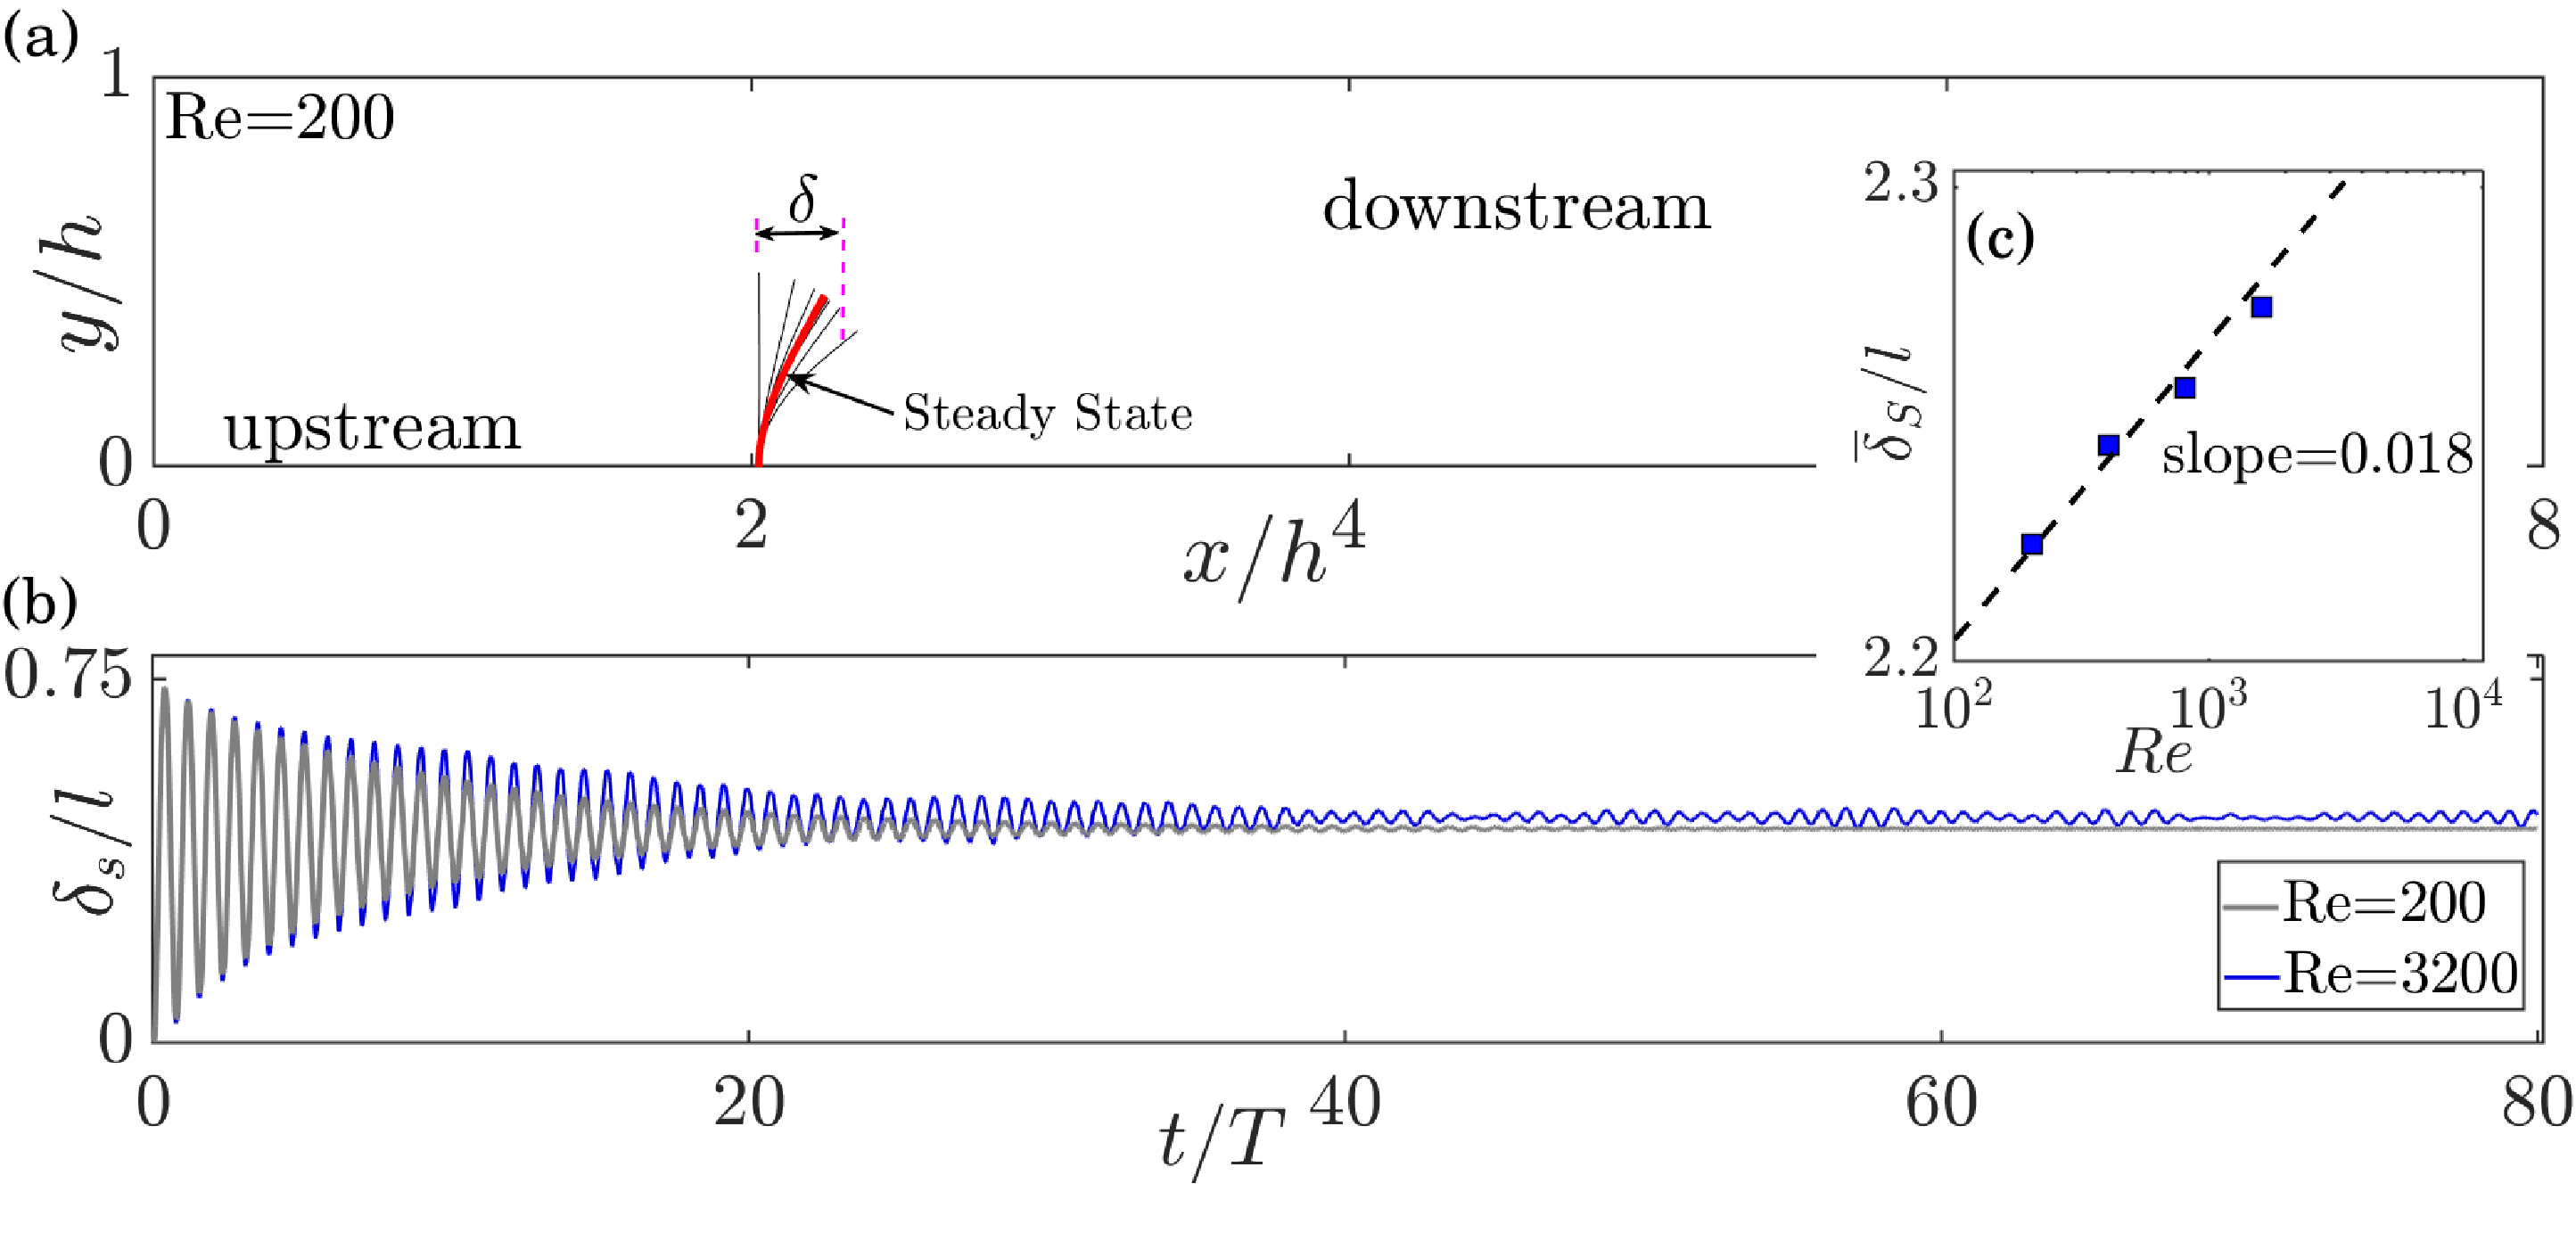
\includegraphics[width=1\linewidth]{Fig03.pdf} 
		\end{minipage} 
		\caption{Single plate dynamics in a channel flow: (a) Filament position on x-y plane at different times for $Re=200$. Thick line for the steady-state shape. (b) tip deflection of a single plate ($\delta_S$) with time. Light gray line for $Re=200$ and blue (dark gray) line for $Re=3200$. (c) steady-state tip deflection ($\overline{\delta}_S$) vs. $Re$. A least square fit gives $(\overline{\delta}_S/l)\propto Re^{0.018}$.}
		\label{fig:Sfil_dyn}
	\end{figure} 
	
	
	\begin{figure}[b]
		\begin{minipage}[c]{0.8\linewidth}
			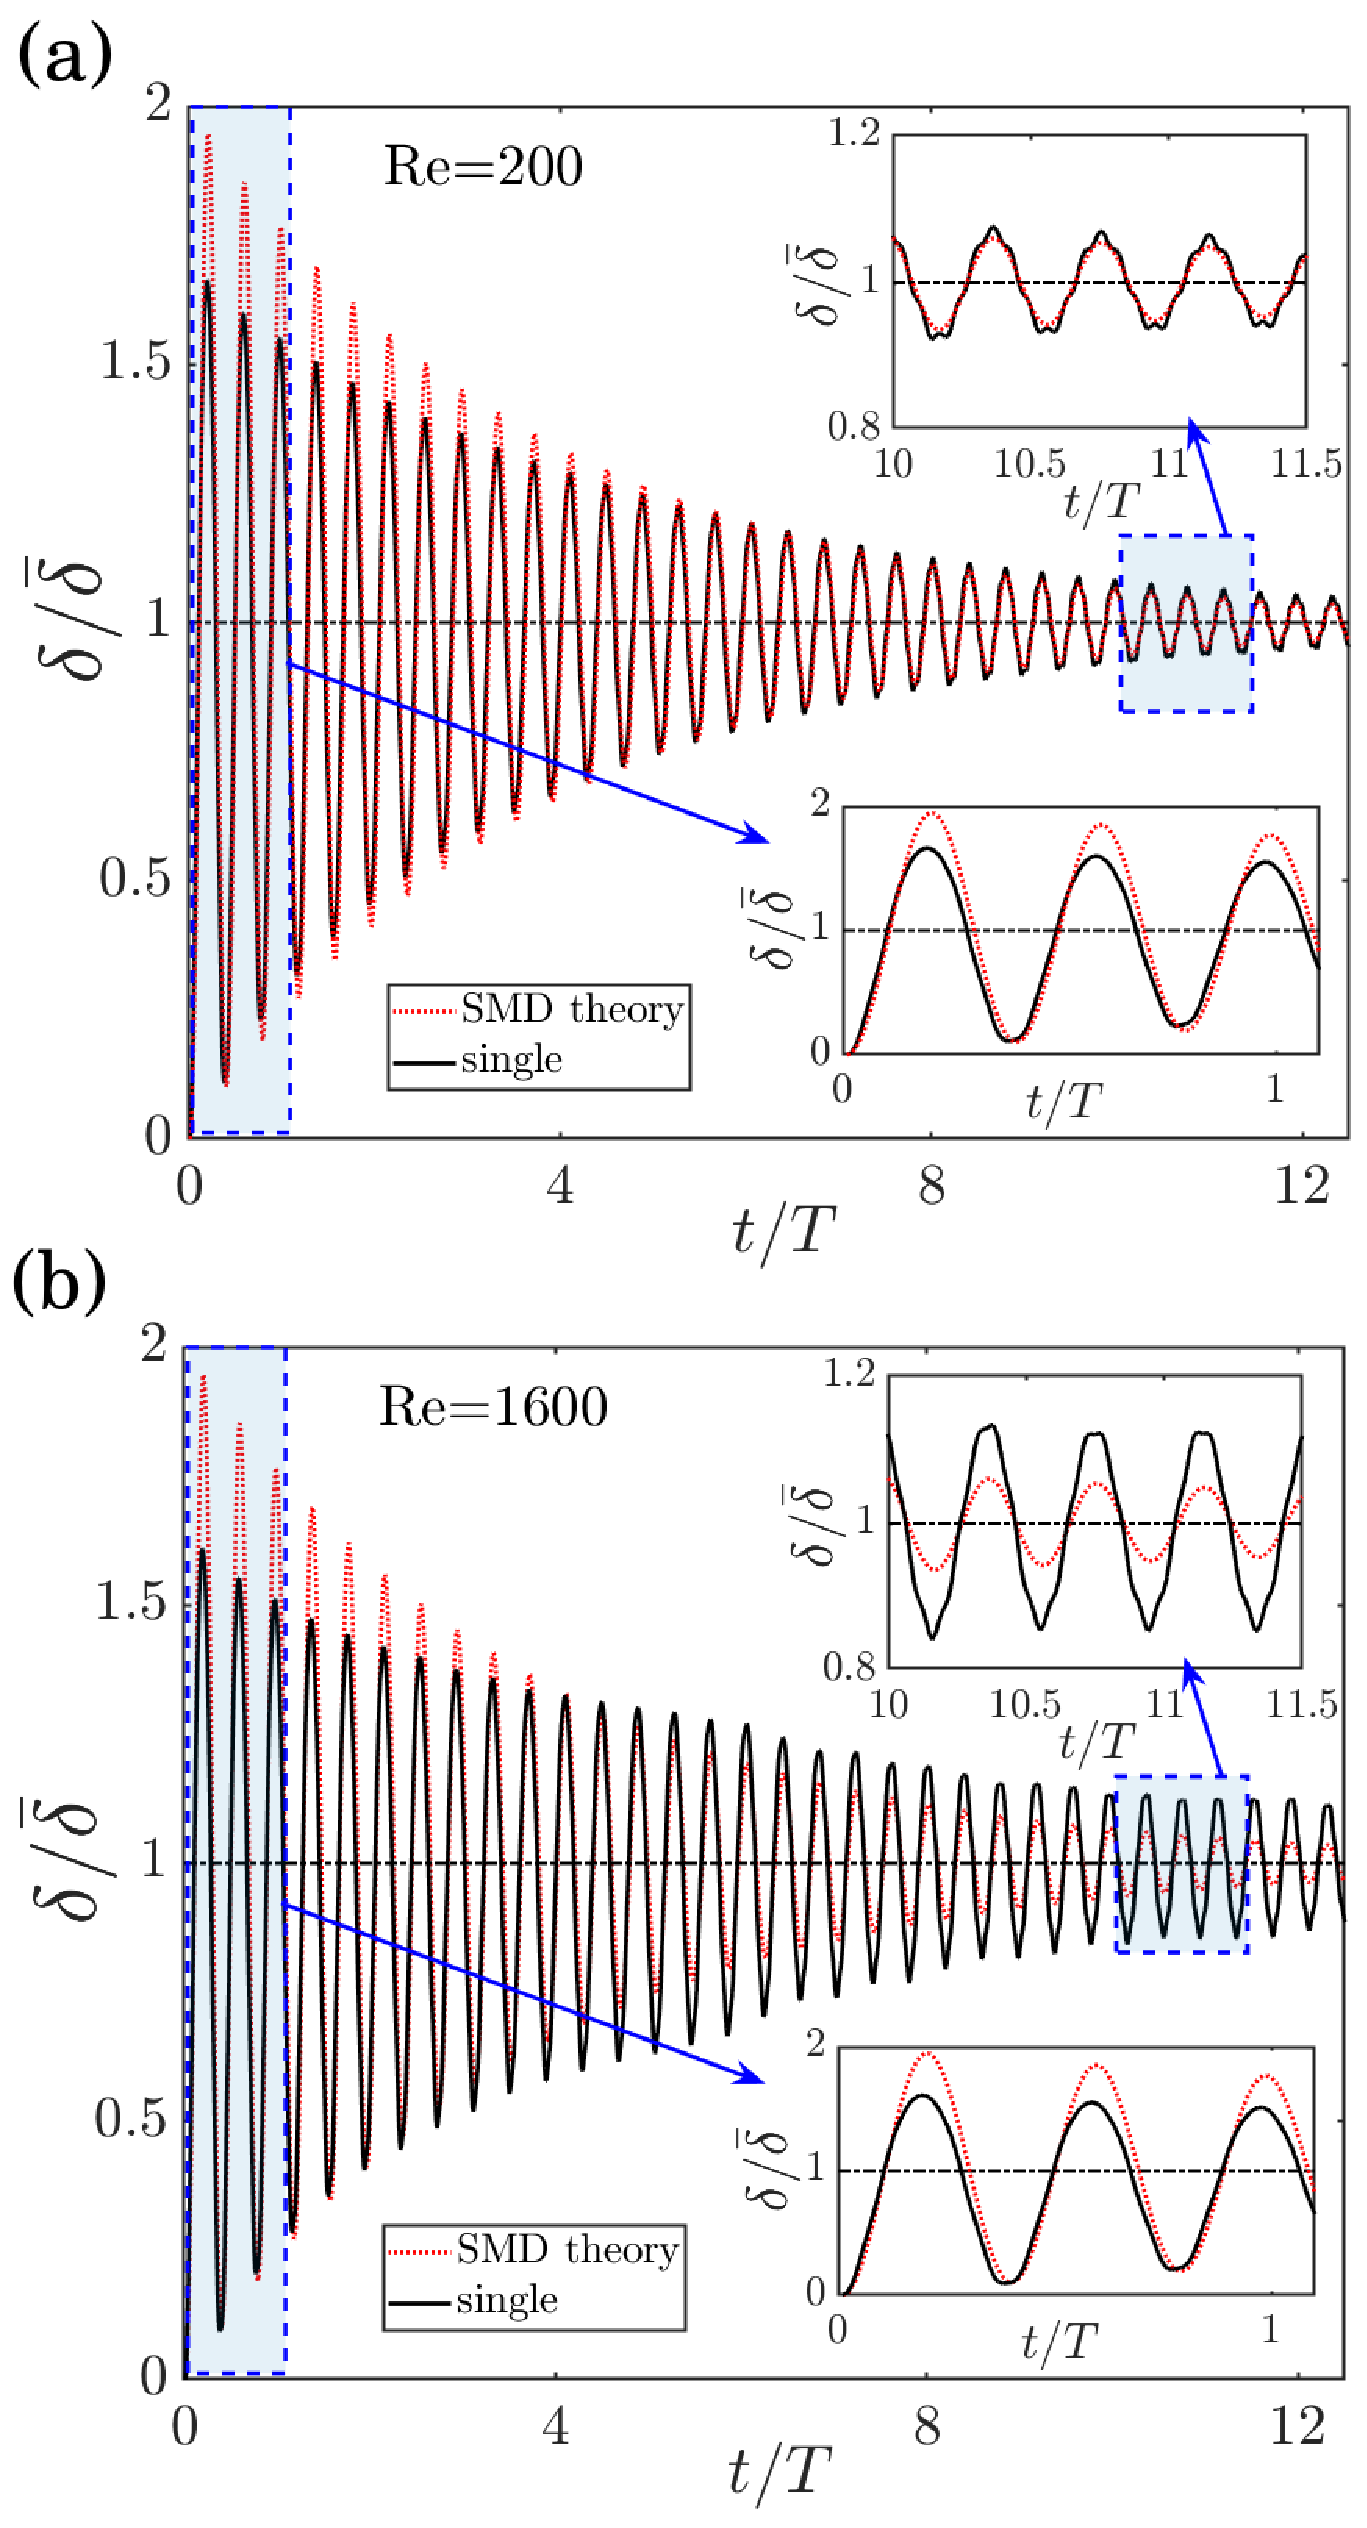
\includegraphics[width=1\linewidth]{Fig04.pdf} 
		\end{minipage} 
		\caption{Normalized tip deflection ($\delta/\overline{\delta}$) vs. dimensionless time ($t/T$) in case of a single plate anchored in a channel flow: (a) for $Re=200$, and (b) for $Re=1600$. Here, $\overline{\delta}$ is the steady-state tip deflection. Dotted line represents the SMD theory and dark solid line represents the FSI simulations. Insets for both initial transients and steady-state response.}
		\label{damping_singlefil}
	\end{figure}
	
	
	
	
	\begin{figure}
		\begin{minipage}[c]{1\linewidth}
			\includegraphics[width=1\linewidth]{Fig05.pdf} 
		\end{minipage} 
		\caption{Two plate dynamics in a channel flow for the plate gap $d/h=2$: (a) the plate shapes on x-y plane at different times for $Re=200$. Thick line for the steady-state shape. (b) Tip deflection of a plate 1 with time, and (c) tip deflection of a plate 2 with time.  Light gray line for $Re=200$ and blue (dark gray) line for $Re=3200$. Inset: tip deflection at plate 2 shows a beat-like pattern.}
		\label{fig:Dfil_dyn_dh2}
	\end{figure}
	
	
	
	
	\begin{figure}
		\begin{minipage}[c]{0.80\linewidth}
			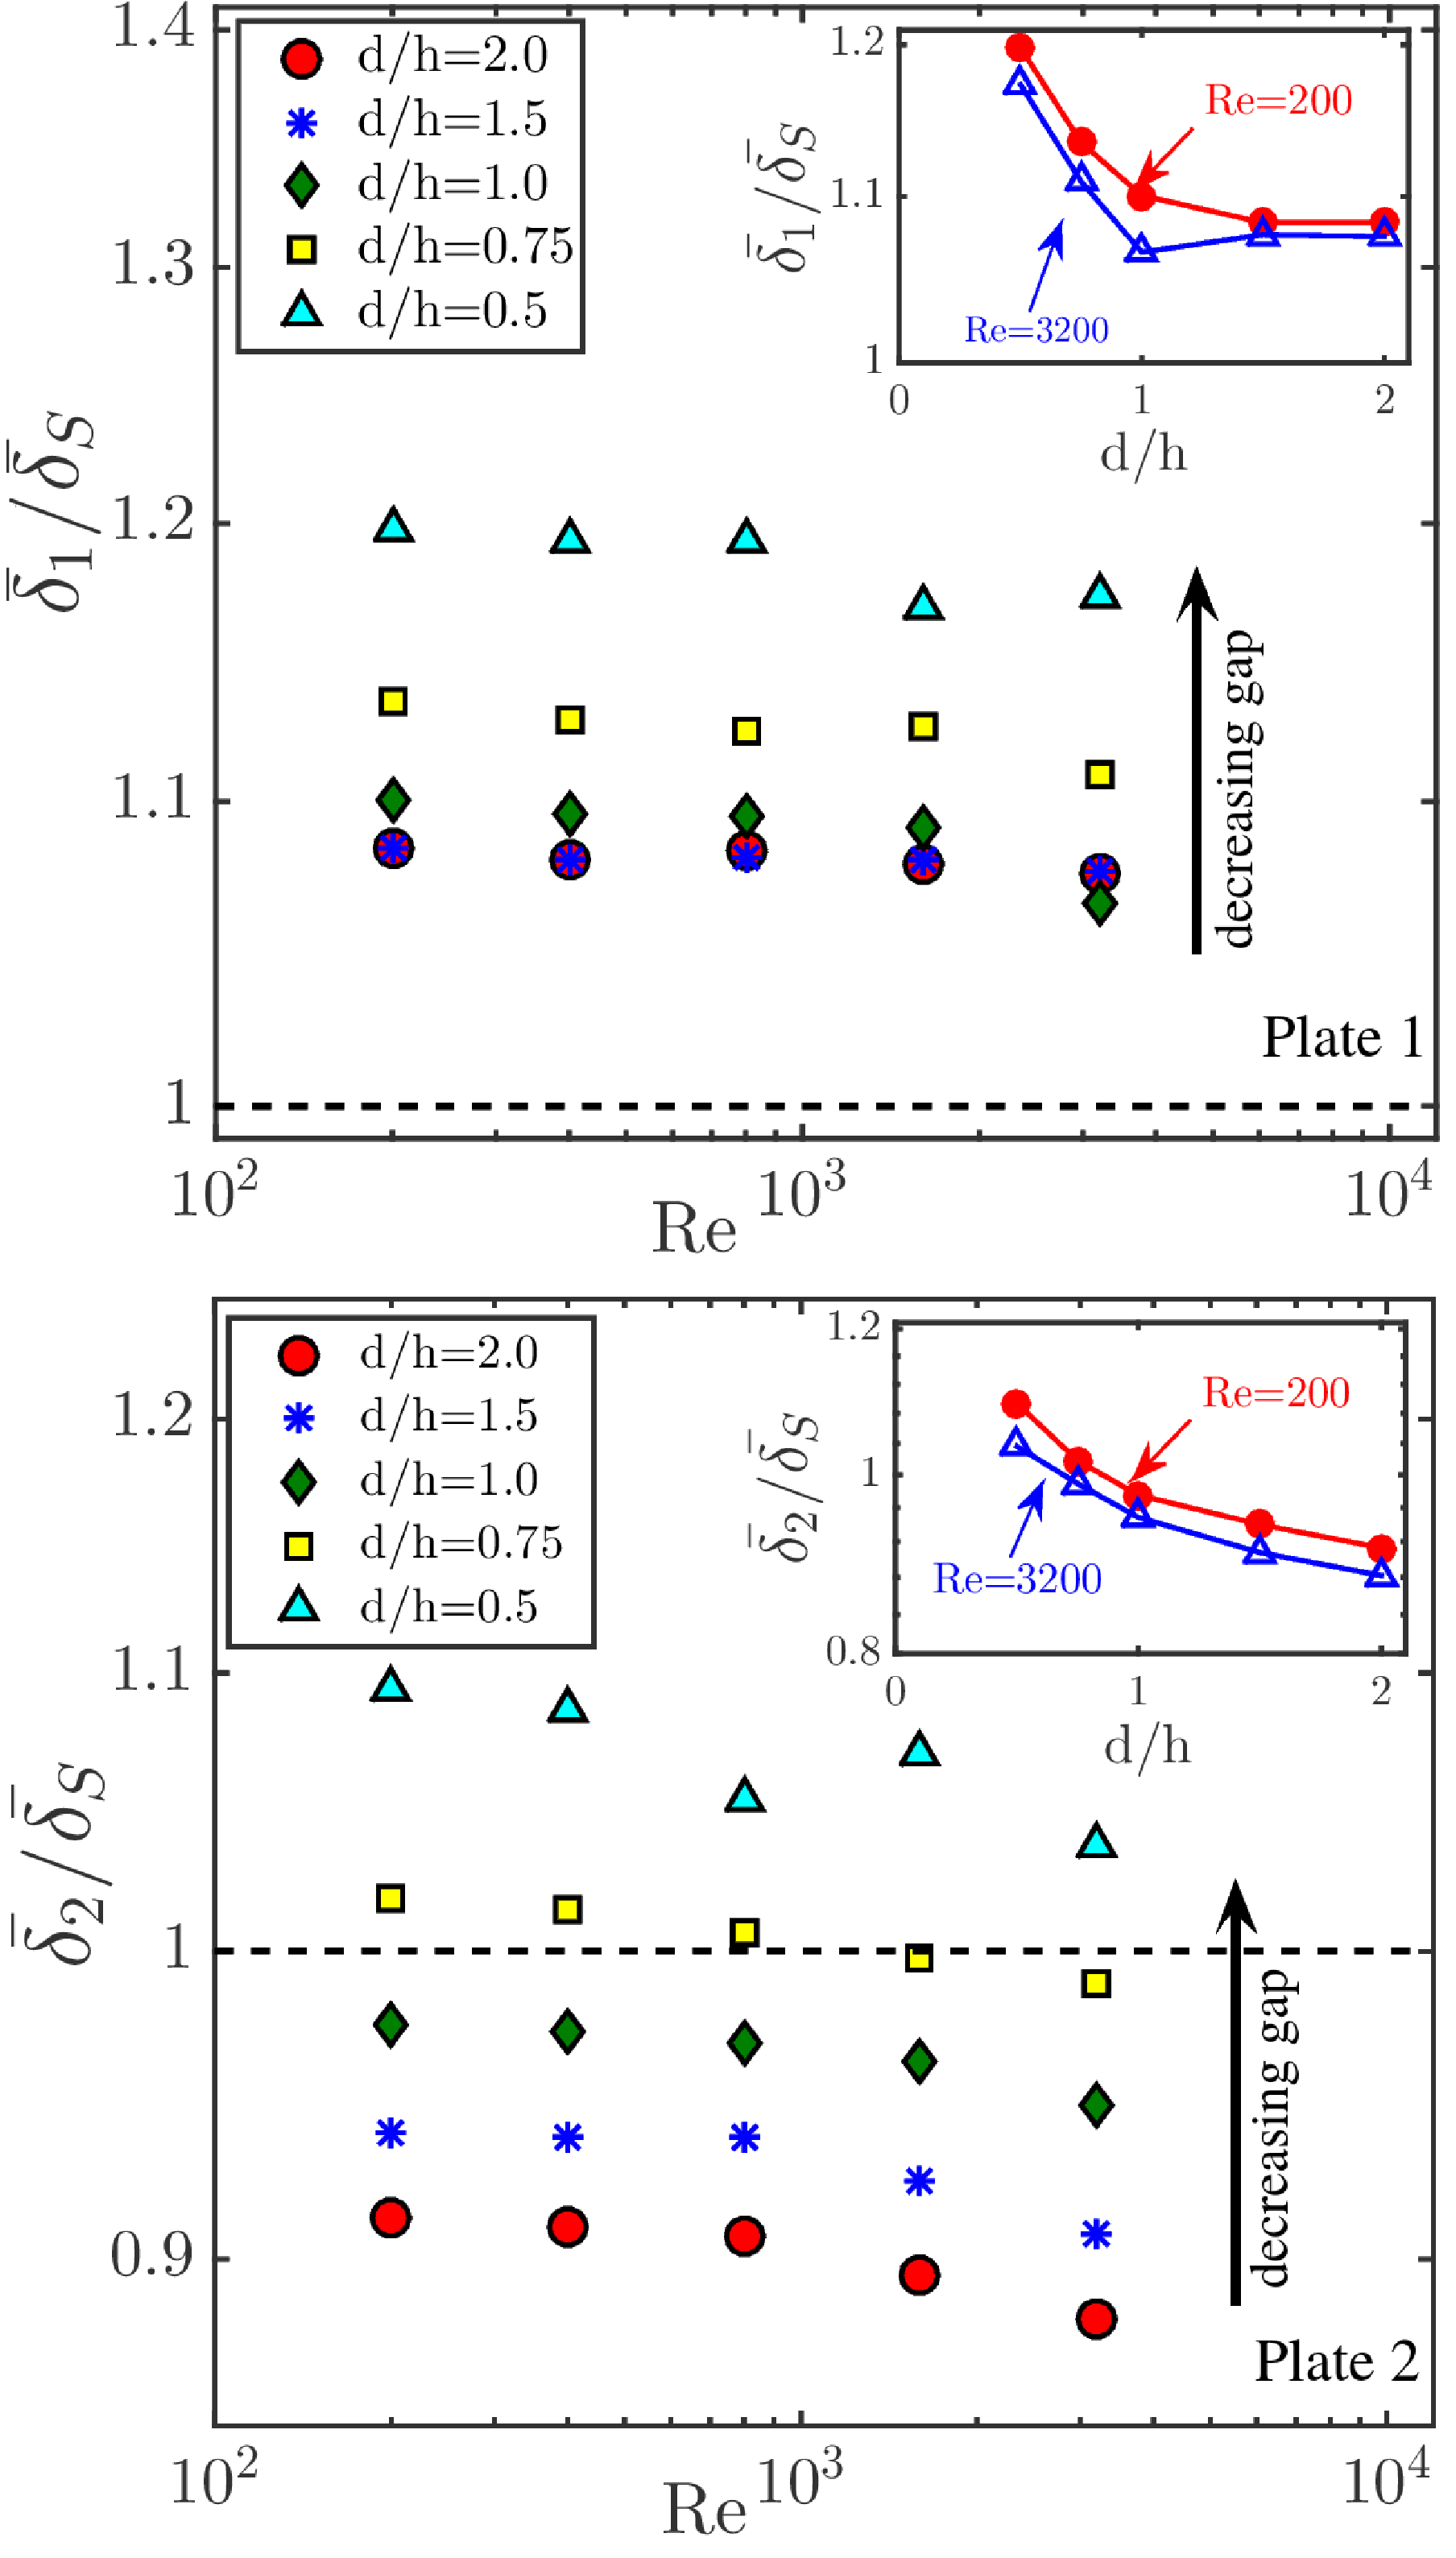
\includegraphics[width=1\linewidth]{Fig06.pdf} 
		\end{minipage} 
		\caption{Time averaged tip deflection vs. $Re$ (a) for plate 1, and (b) for plate 2. Symbols are circles ($d/h=2$), stars ($d/h=1.5$), diamonds ($d/h=1$), squares ($d/h=0.75$) and triangles ($d/h=0.5$). Insets for the normalized tip deflections vs. the plate gap at two different $Re$}
		\label{fig:steady_double_vs_Re}
	\end{figure} 
	
	
	\section{Structural response}
	
	
	
	\begin{figure*}
		\begin{minipage}[c]{0.85\linewidth}
			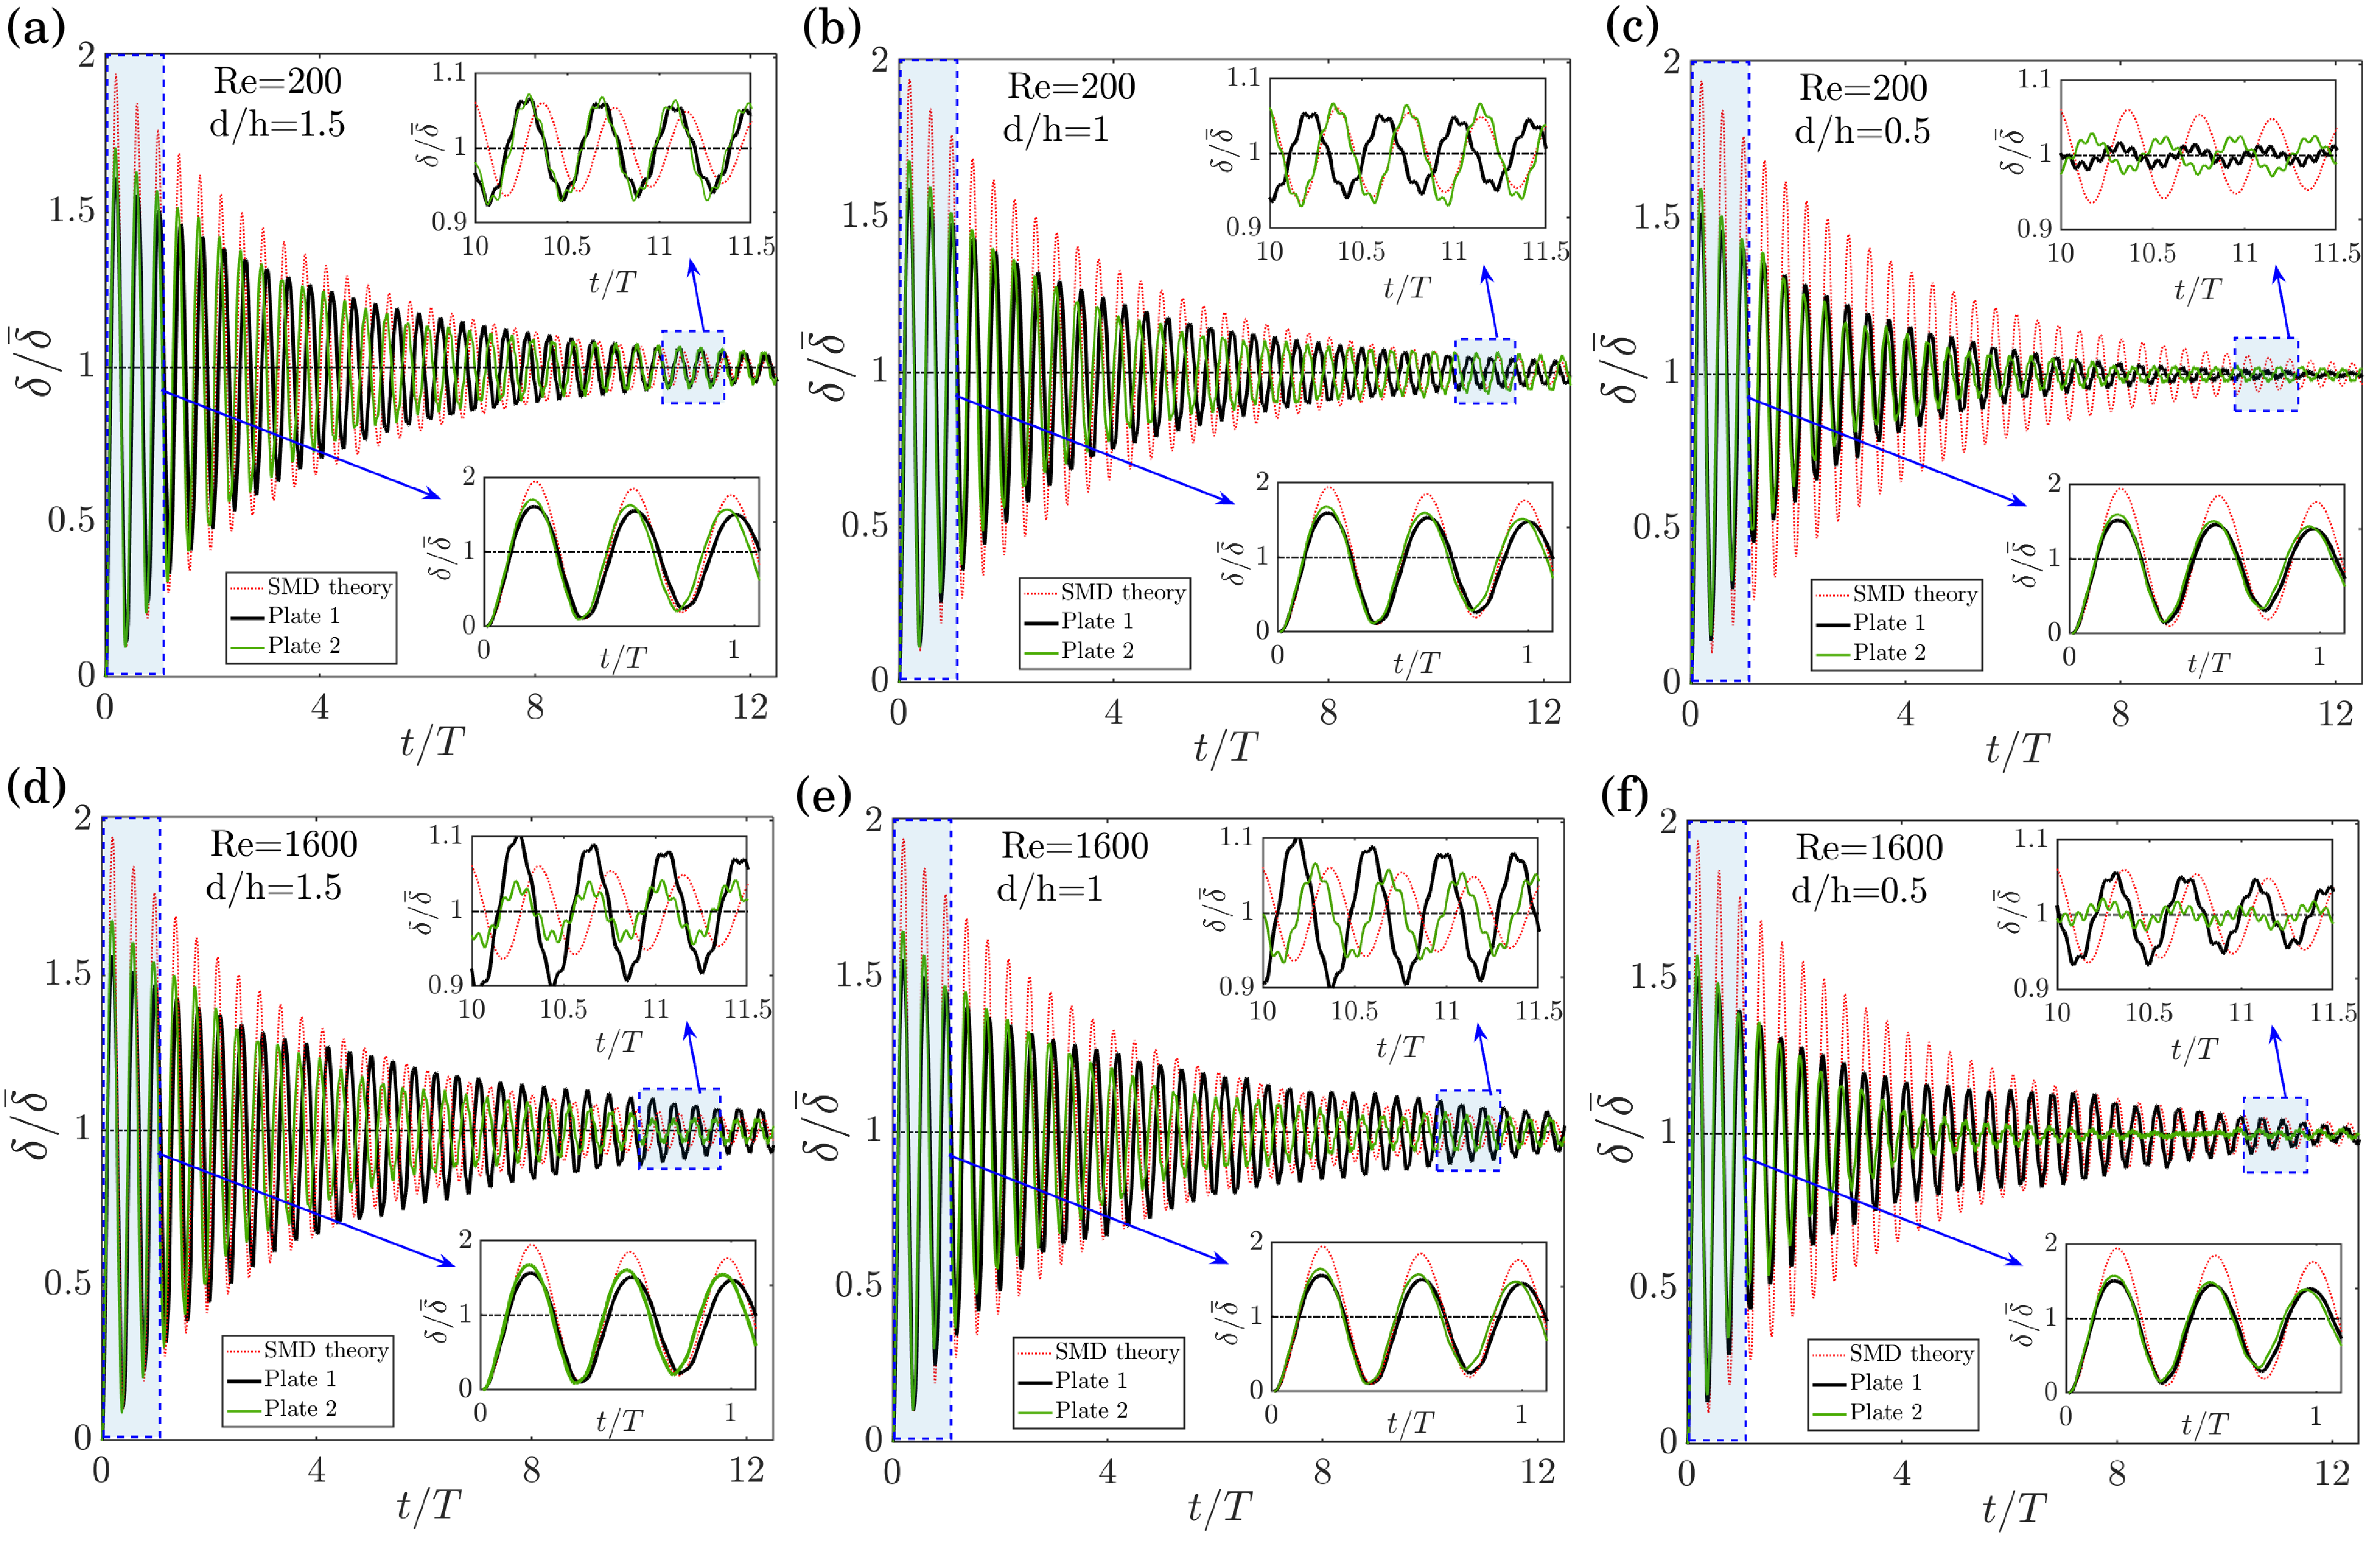
\includegraphics[width=1\linewidth]{Fig07.pdf} 
		\end{minipage} 
		\caption{Normalized tip deflections vs. dimensionless time: Top panels (a, b and c) for $Re=200$ and bottom panels (d, e and f) for $Re=1600$. The plate gaps are $d/h=2$ (in panels a and d), $d/h=1$ (in panels b and e), and $d/h=0.5$ (in panels c and f). Dotted line for the SMD theory, black solid line for the plate 1 and green (gray) line for the plate 2. Insets for tip deflections both at the initial transients and at the steady-state.}
		\label{fig:transient_double_vs_Re}
	\end{figure*} 
	
	In figure~\ref{fig:Sfil_dyn}a, shape oscillations of the single plate for $Re=200$ are shown, where the plate acts like a `cantilever'. In figure~\ref{fig:Sfil_dyn}b, instantaneous tip deflection in the streamwise direction, $\delta_S=x_{tip}(t)-x_{tip}(t=0)$, is shown. The deflection shows under-damped oscillatory behavior with time, and eventually the plate settles to a steady-state for $t>50T$. The time-averaged tip deflection of the single plate, $\overline{\delta}_S$ as a function of $Re$, is shown in figure~\ref{fig:Sfil_dyn}c. We found $\overline{\delta}_S\propto Re^{0.018}$. In our work, the steady-state time-averages are computed in a range $50T$ to $200T$, which is considered to be very long in comparison to the plates' natural oscillation period.
	
	The plate bends in the streamwise direction and is set into oscillations due to the hydrodynamic impact. The resulting tip deflection can be understood better by using a spring-mass-damper (SMD) theory-based model~\cite{Kelley2004}. In this model, the plate is assumed as a lumped mass subjected to a point load with one-degree of freedom. Any other high-dimensional models based on the continuum theory can provide accurate results, but require complete information on the fluid-structure interaction in prior. In the SMD theory, the tip deflection $\delta(t)$ satisfies a second-order differential equation of the form $\ddot{\delta}+2\zeta\omega\dot{\delta}+\omega^2 \delta=F$. Here, the over-dot corresponds to the differentiation with time, $\zeta$ is the damping ratio, $\omega$ is the natural frequency, and $F$ is the applied load. The plate's first natural frequency based on the Euler-Bernoulli's beam theory is expressed as $\omega=\left(\pi/\sqrt{3}\right)^2\sqrt{\mathcal{E}I/(\rho_s bwl^4)}$, see~\cite{Kelley2004}. We have used $F=0$ for $t\le 0$, and $F=\omega^2$ for $t>0$, to mimic the hydrodynamic impact on the plate. The tip deflection satisfies, $\delta(t) = \overline{\delta} -\overline{\delta}\left[e^{-\zeta \omega t}\,{sin(\sqrt{1-\zeta^2} \omega t+\phi)\over sin(\phi)}\right]$, where $\overline{\delta}$ is the time-averaged tip deflection and $\phi=cos^{-1}(\zeta)$ is the phase angle. In our work, the damping ratio of the plate is $\zeta=0.0175$, and the oscillations are under-damped.\\
	
	
	
	
	In figure~\ref{damping_singlefil}, the normalized tip deflection for the single plate ($\delta/\overline{\delta}$) calculated from our simulations, and response based on the SMD theory are compared. At the initial time, the tip deflections in our simulations show underdamped sinusoidal behaviour. However, at large time, the deflection shows non-sinusoidal behaviour with cusp-like shape. Eventually, the oscillations are dampened by the fluid viscosity.
	
	In figure~\ref{fig:Dfil_dyn_dh2}, the tip oscillations in the case of a double plate configuration are shown. At low $Re~(\le200)$, the oscillating plates attain a steady-state within $50T$. However, at high $Re~(\approx3200)$, vortices detach regularly from the plates' tip, and that reflect as the self-sustaining tip oscillations for a long time. We found intriguing features such as the nearly periodic response of the plate 1, and the beat-like response of the plate 2 (see inset in figure~\ref{fig:Dfil_dyn_dh2}c). From information on vortices (mentioned in section V), we observe that the primary vortices which detach at the plate 1 strike the plate 2 and generate additional (secondary) vortices in the downstream. This complex coupling between the primary and the secondary vortices leads to an uneven distribution of hydrodynamic load on the plate 2, and hence, we observe a beat-like response.
	
	In figure~\ref{fig:steady_double_vs_Re}, steady-state time-averaged tip deflections of the plate 1 (denoted as $\overline{\delta}_1$) and the plate 2 (denoted as $\overline{\delta}_2$) for a double plate configuration are shown. The single plate's steady-state tip deflection $\overline{\delta}_S$, serves as a reference scale to express the deflections obtained in other configurations. We observe $\overline{\delta_1}>\overline{\delta}_S$, for any given $Re$ and $d/h$. It is worthy of notice that $\overline{\delta}_2 < \overline{\delta}_S$ for $0.8\le d/h<2$, and $\overline{\delta}_2>\overline{\delta}_S$ for $d/h<0.8$. From insets of the same figures, we can notice that the normalized tip deflections increase with decrease in $d/h$.
	
	In figure~\ref{fig:transient_double_vs_Re}, the tip deflections for different $d/h$ are shown. The plates show coherent (in-phase) oscillations for $d/h>1$, and incoherent (out-phase) oscillations for $d/h\le1$. The regular detachment of vortices causes the plates' to oscillate coherently, whereas, any irregular detachment leads to incoherent plate oscillations. We have not attempted any further quantification of incoherence because of the importance given to the flow features.
	
	
	\section{Flow features behind plates}
	
	
	\subsection{Streamlines}
	
	
	\begin{figure}
		\begin{minipage}[c]{1\linewidth}
			\includegraphics[width=1\linewidth]{Fig08.pdf} 
		\end{minipage} 
		\caption{Streamlines in the channel: (a) single plate, (b) double plates with $d/h=2$, (c) double plates with $d/h=1$, and (d) double plates with $d/h=0$. The flow Reynolds number increase in each panel from $Re=200$ to 3200. The vortex rolls build-up at the plates' tip and get down-washed in the channel. See animation 1. Streamlines are colored with dimensionless velocity, ($v_x/v_{\infty}$). The color bar ranges from -4 (dark blue) to 4 (light red).}
		\label{fig:streamlines}
	\end{figure}
	
	\begin{figure}[b]
		\begin{minipage}{1\linewidth}
			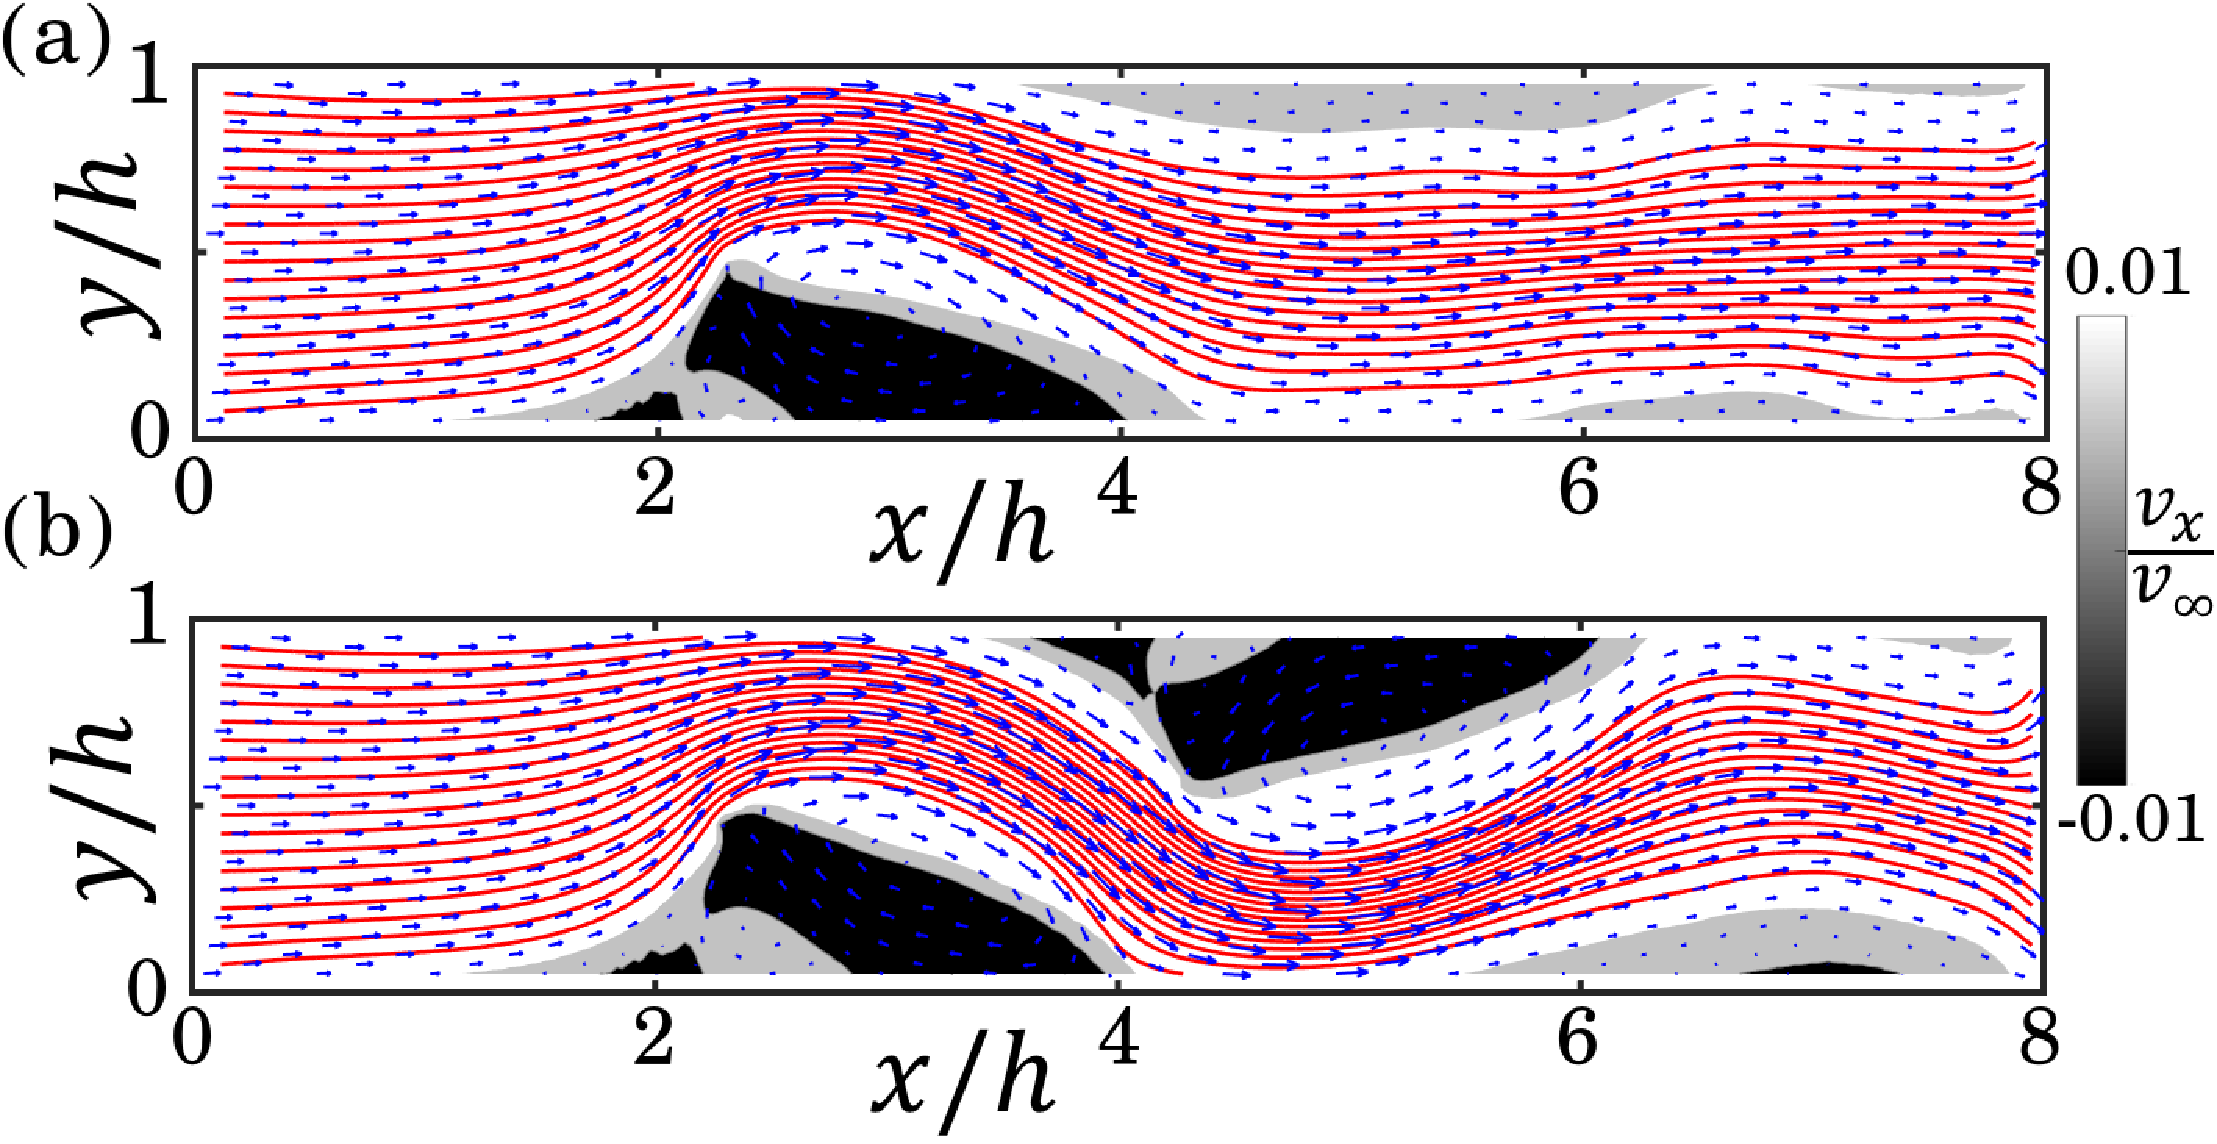
\includegraphics[width=1\linewidth]{Fig09.pdf} 
		\end{minipage} 
		\caption{Time-averaged flow field for $Re=800$. (a) for a single plate case, and (b) for a double plate case with $d/h=2$. The background is colored based on the time-averaged streamwise velocity $v_x$ (in gray scale). The color bar ranges from $-0.01$ (black) to $0.01$ (white).}
		\label{fig:stream_timeavg}
	\end{figure}
	
	\begin{figure}
		\begin{minipage}[c]{1\linewidth}
			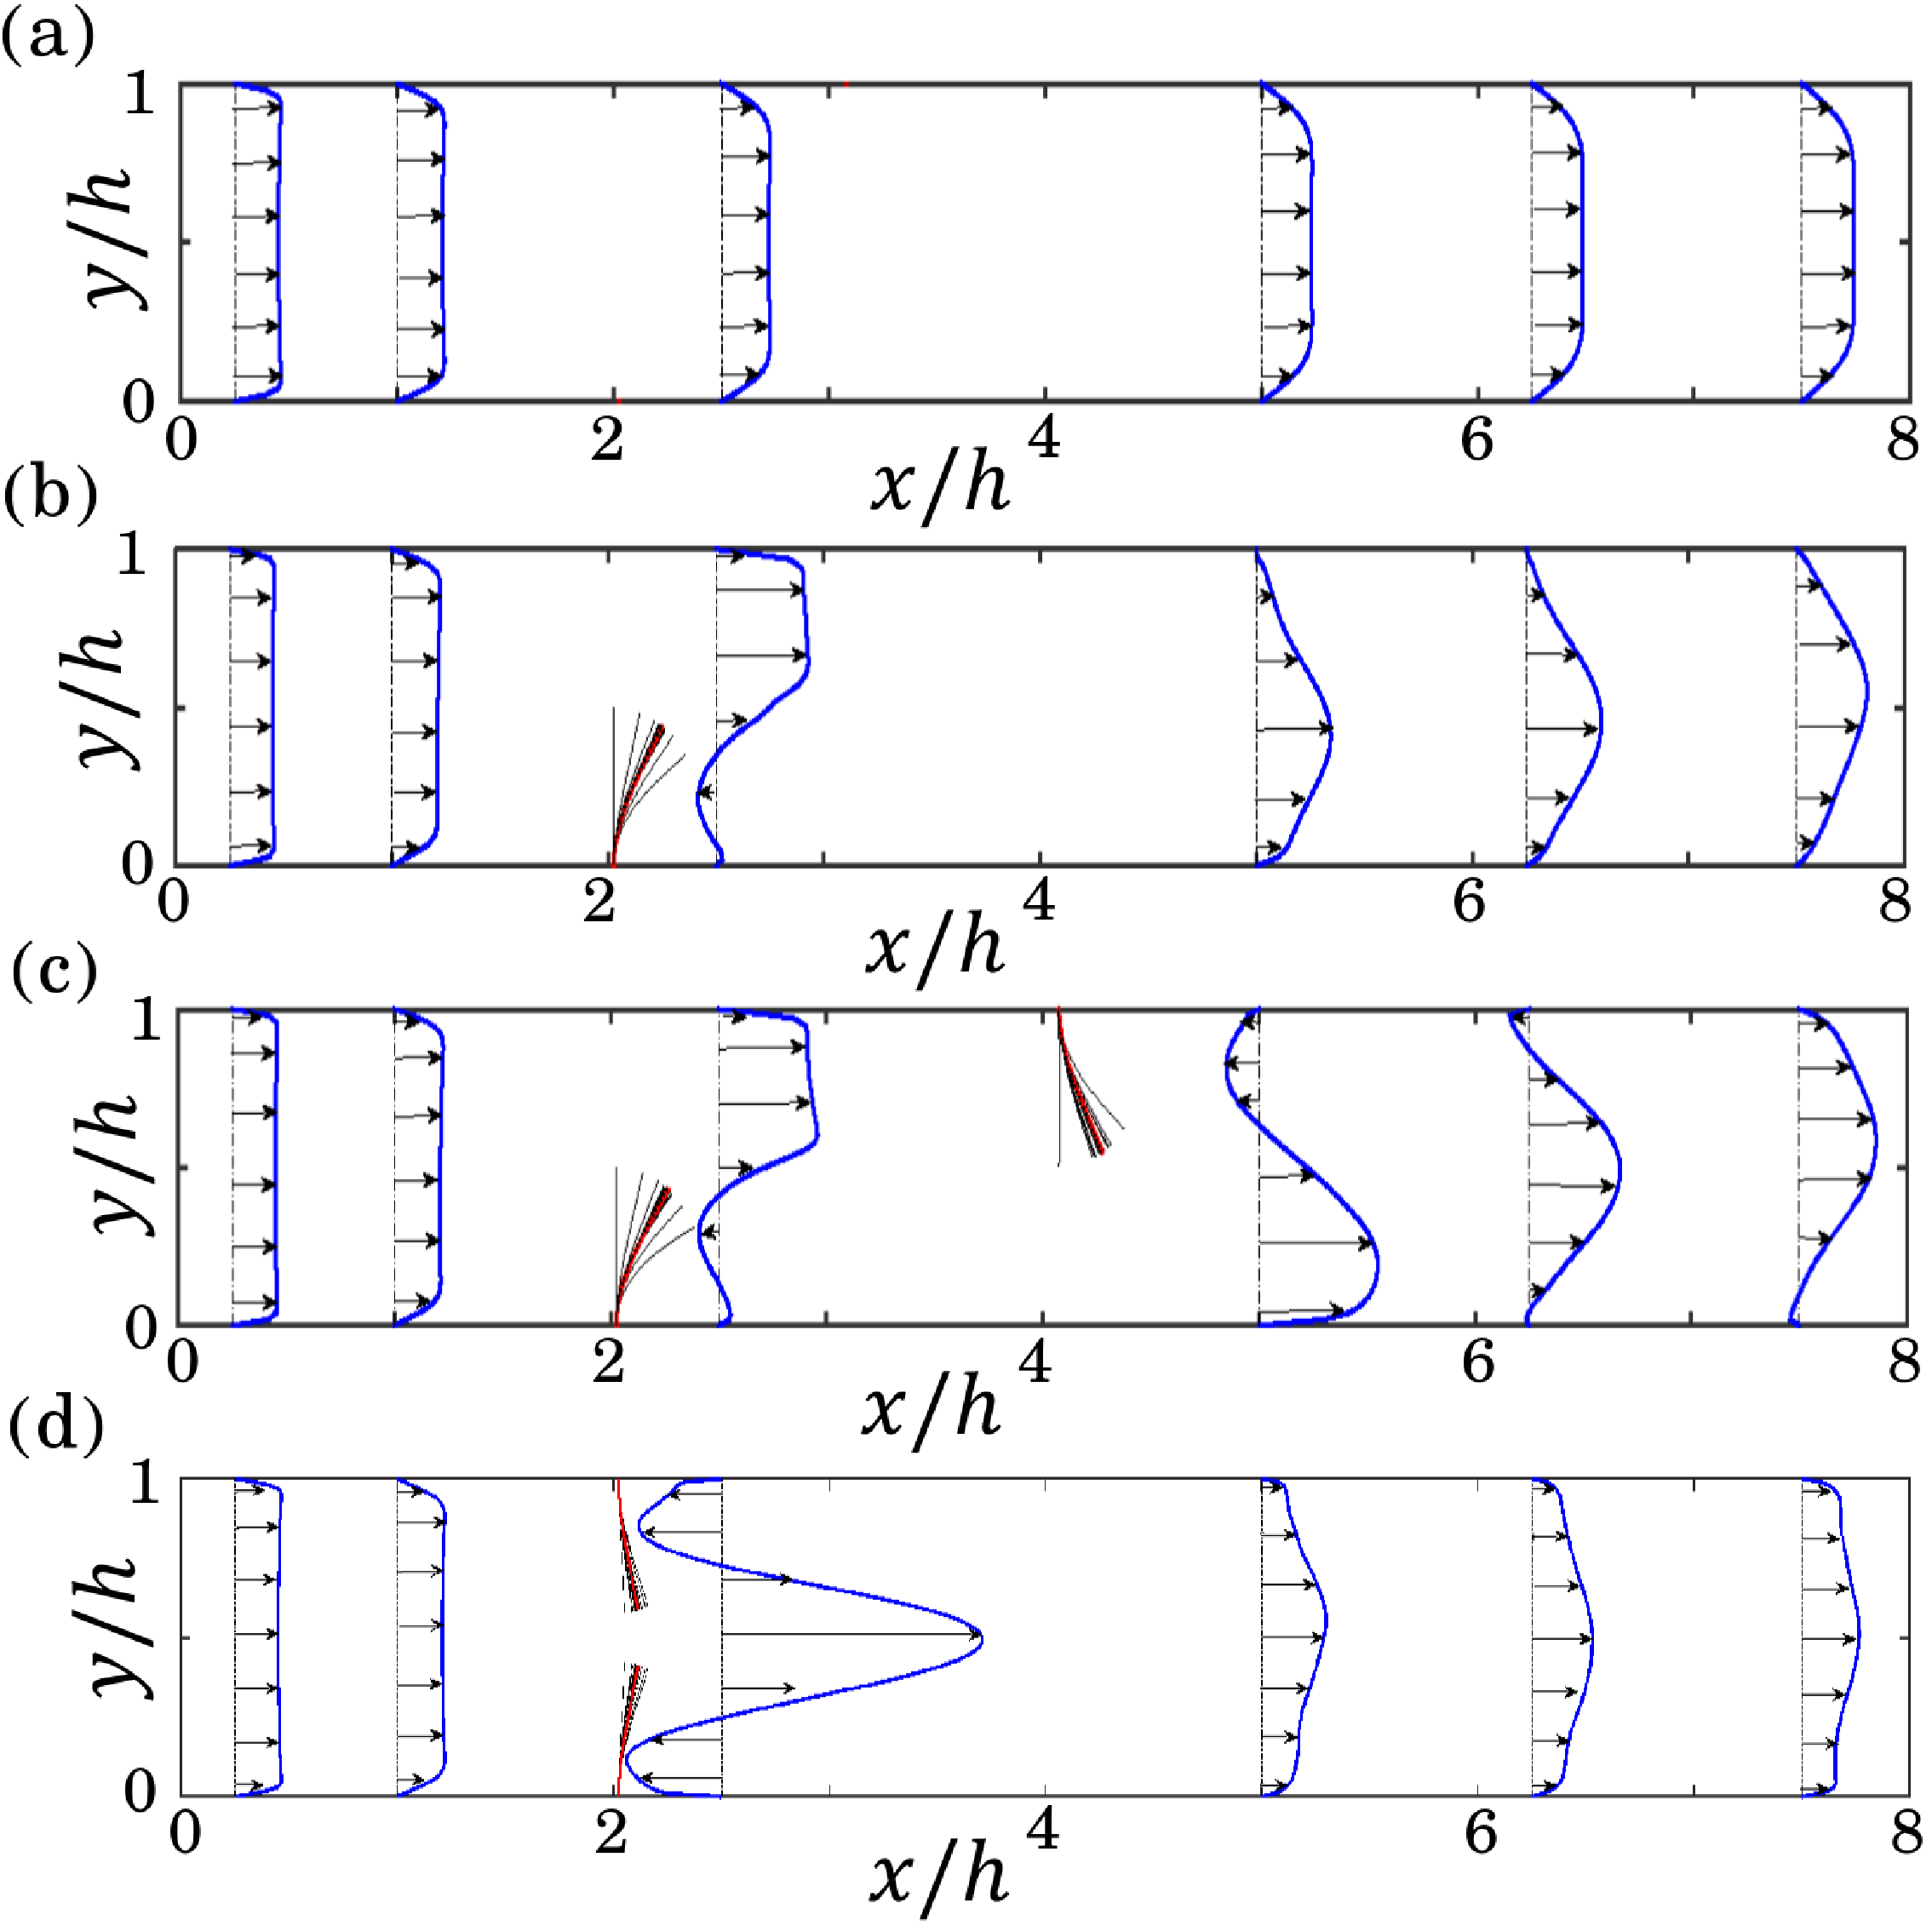
\includegraphics[width=1\linewidth]{Fig10.pdf} 
		\end{minipage} 
		\caption{Time-averaged velocity profiles across the channel at six different streamwise locations. Panels for a channel: (a) without plates (b) with a single plate, (c) with two plates with gap $d/h=2$, and (d) with two plates with gap $d/h=0$. Simulations for $Re=800$.}
		\label{fig:vel_prof_timeavg}
	\end{figure}
	
	
	In our simulations, the flow enters the channel from the inlet, passes over the plates by bending them, and finally exits through the outlet (see figure~\ref{fig:schematic}). The top-bottom flow symmetry (as expected in a plane channel flow at low $Re$) breaks with the presence of a plate (see figure~\ref{fig:streamlines}a). Vortices can be observed next to the plates in the downstream side, and their size is determined by the competition between the convective motions and the viscous diffusion. At low $Re$, growth of the tip-generated vortices is inhibited by the diffusion process, whereas, at high $Re$, the convective motions dominate, and cause the vortices (or rolls) to detach from the plates' tip (see animation 1). The detached vortices possess momentum in both streamwise and crosswise directions, so, the flow meanders in the downstream.
	
	The streamlines for $d/h=2$ and $d/h=1$ are shown in figure~\ref{fig:streamlines}b and in~\ref{fig:streamlines}c, respectively. On decreasing the $d/h$, the flow accelerates in the gap to maintain the mass conservation. The primary vortex (present next to the plate 1) stays confined between the plates and strengthens in circulation with time. Another (secondary) vortex generates next to plate 2 and causes the flow meandering in the downstream. With the increase in $Re$, the disturbance level in the flow also increases, and hence, many small scale vortices are developed.
	
	In figure~\ref{fig:streamlines}d, streamlines for the zero gap i.e., ($d/h=0$) are shown. The flow coming out through the two plates, in this case, mimics a classical jet-like stream. However, due to the plate oscillations, puff like ejections are observed at regular times. At very low $Re$, the detached vortices do not interact with each other, so a symmetric jet is observed. With an increase in $Re$, the vortices interact with each other, and hence, an asymmetric oscillatory jet is observed. We observed that the vortices are spatially aligned along the channel length with a periodicity of one roll per $h$ length.
	
	
	\subsection{Time-averaged velocity profiles and wall gradients}
	
	
	\begin{figure}
		\begin{minipage}[c]{1\linewidth}
			\includegraphics[width=1\linewidth, height=11cm]{Fig11.pdf} 
		\end{minipage} 
		\caption{Time-averaged center-line Reynolds number ($Re_c$) along the channel's length. Panels: (a) when the inlet flow $Re=800$ and (b) when inlet flow $Re=3200$. In panels c and d, $Re_c$ in a double plate configuration is normalized with $Re_c$ of a single plate configuration ($Re_{cS}$). To guide eye, dotted lines show the flow blockage zone.}
		\label{fig:Vcentre_vs_x}
		\vspace{0cm}
	\end{figure}
	
	
	In figure~\ref{fig:stream_timeavg}, time-averaged flow fields in the case of a single plate and a double plate configuration are shown. We can observe recirculation zones attached to the plates in the downstream side. Few noteworthy observations when comparing the double and the single plate configuration are, constriction of the primary recirculation zone between the two plates, stronger secondary recirculation zone next to the plate 2, and increase in wavy nature of the mean flow.
	
	
	In figure~\ref{fig:vel_prof_timeavg}, time-averaged streamwise velocities across the channel, at six different streamwise locations, are shown. As mentioned earlier, flow develops continuously throughout the channel length. The velocity profiles near the entrance region show top-bottom symmetry with the maximum velocity at the channel center. However, the observed symmetry in the flow breaks near the plates. In the downstream side, spatial undulations in the flow are observed. The symmetry in the flow can be restored if the two plates are aligned on the opposite walls, i.e., for $d/h=0$.
	
	
	As mentioned earlier, to maintain the mass continuity, the flow has to accelerate in the gap between the plates. To test this rationale, the local flow Reynolds number along the channel center-line, $Re_c=\overline{v}_xl/\nu$ (which is calculated at $y=0.5h$) is shown in figure~\ref{fig:Vcentre_vs_x}. We can notice that $Re_c$ varies non-monotonically along the channel centerline. We have compared the local $Re_c$ variation in a double plate configuration to the same in a single plate configuration ($Re_{cS}$) in figures~\ref{fig:Vcentre_vs_x}c and \ref{fig:Vcentre_vs_x}d. It is worth noticing that the double plate configuration can accelerate the flow to a much high level (four to six times) when compared to either a plane channel or a single plate case.
	
	
	\section{Flow frequency and vortex structures}
	
	\subsection{Wake characteristics and flow frequencies}
	
	
	\begin{figure}[b]
		\begin{minipage}[c]{1\linewidth}
			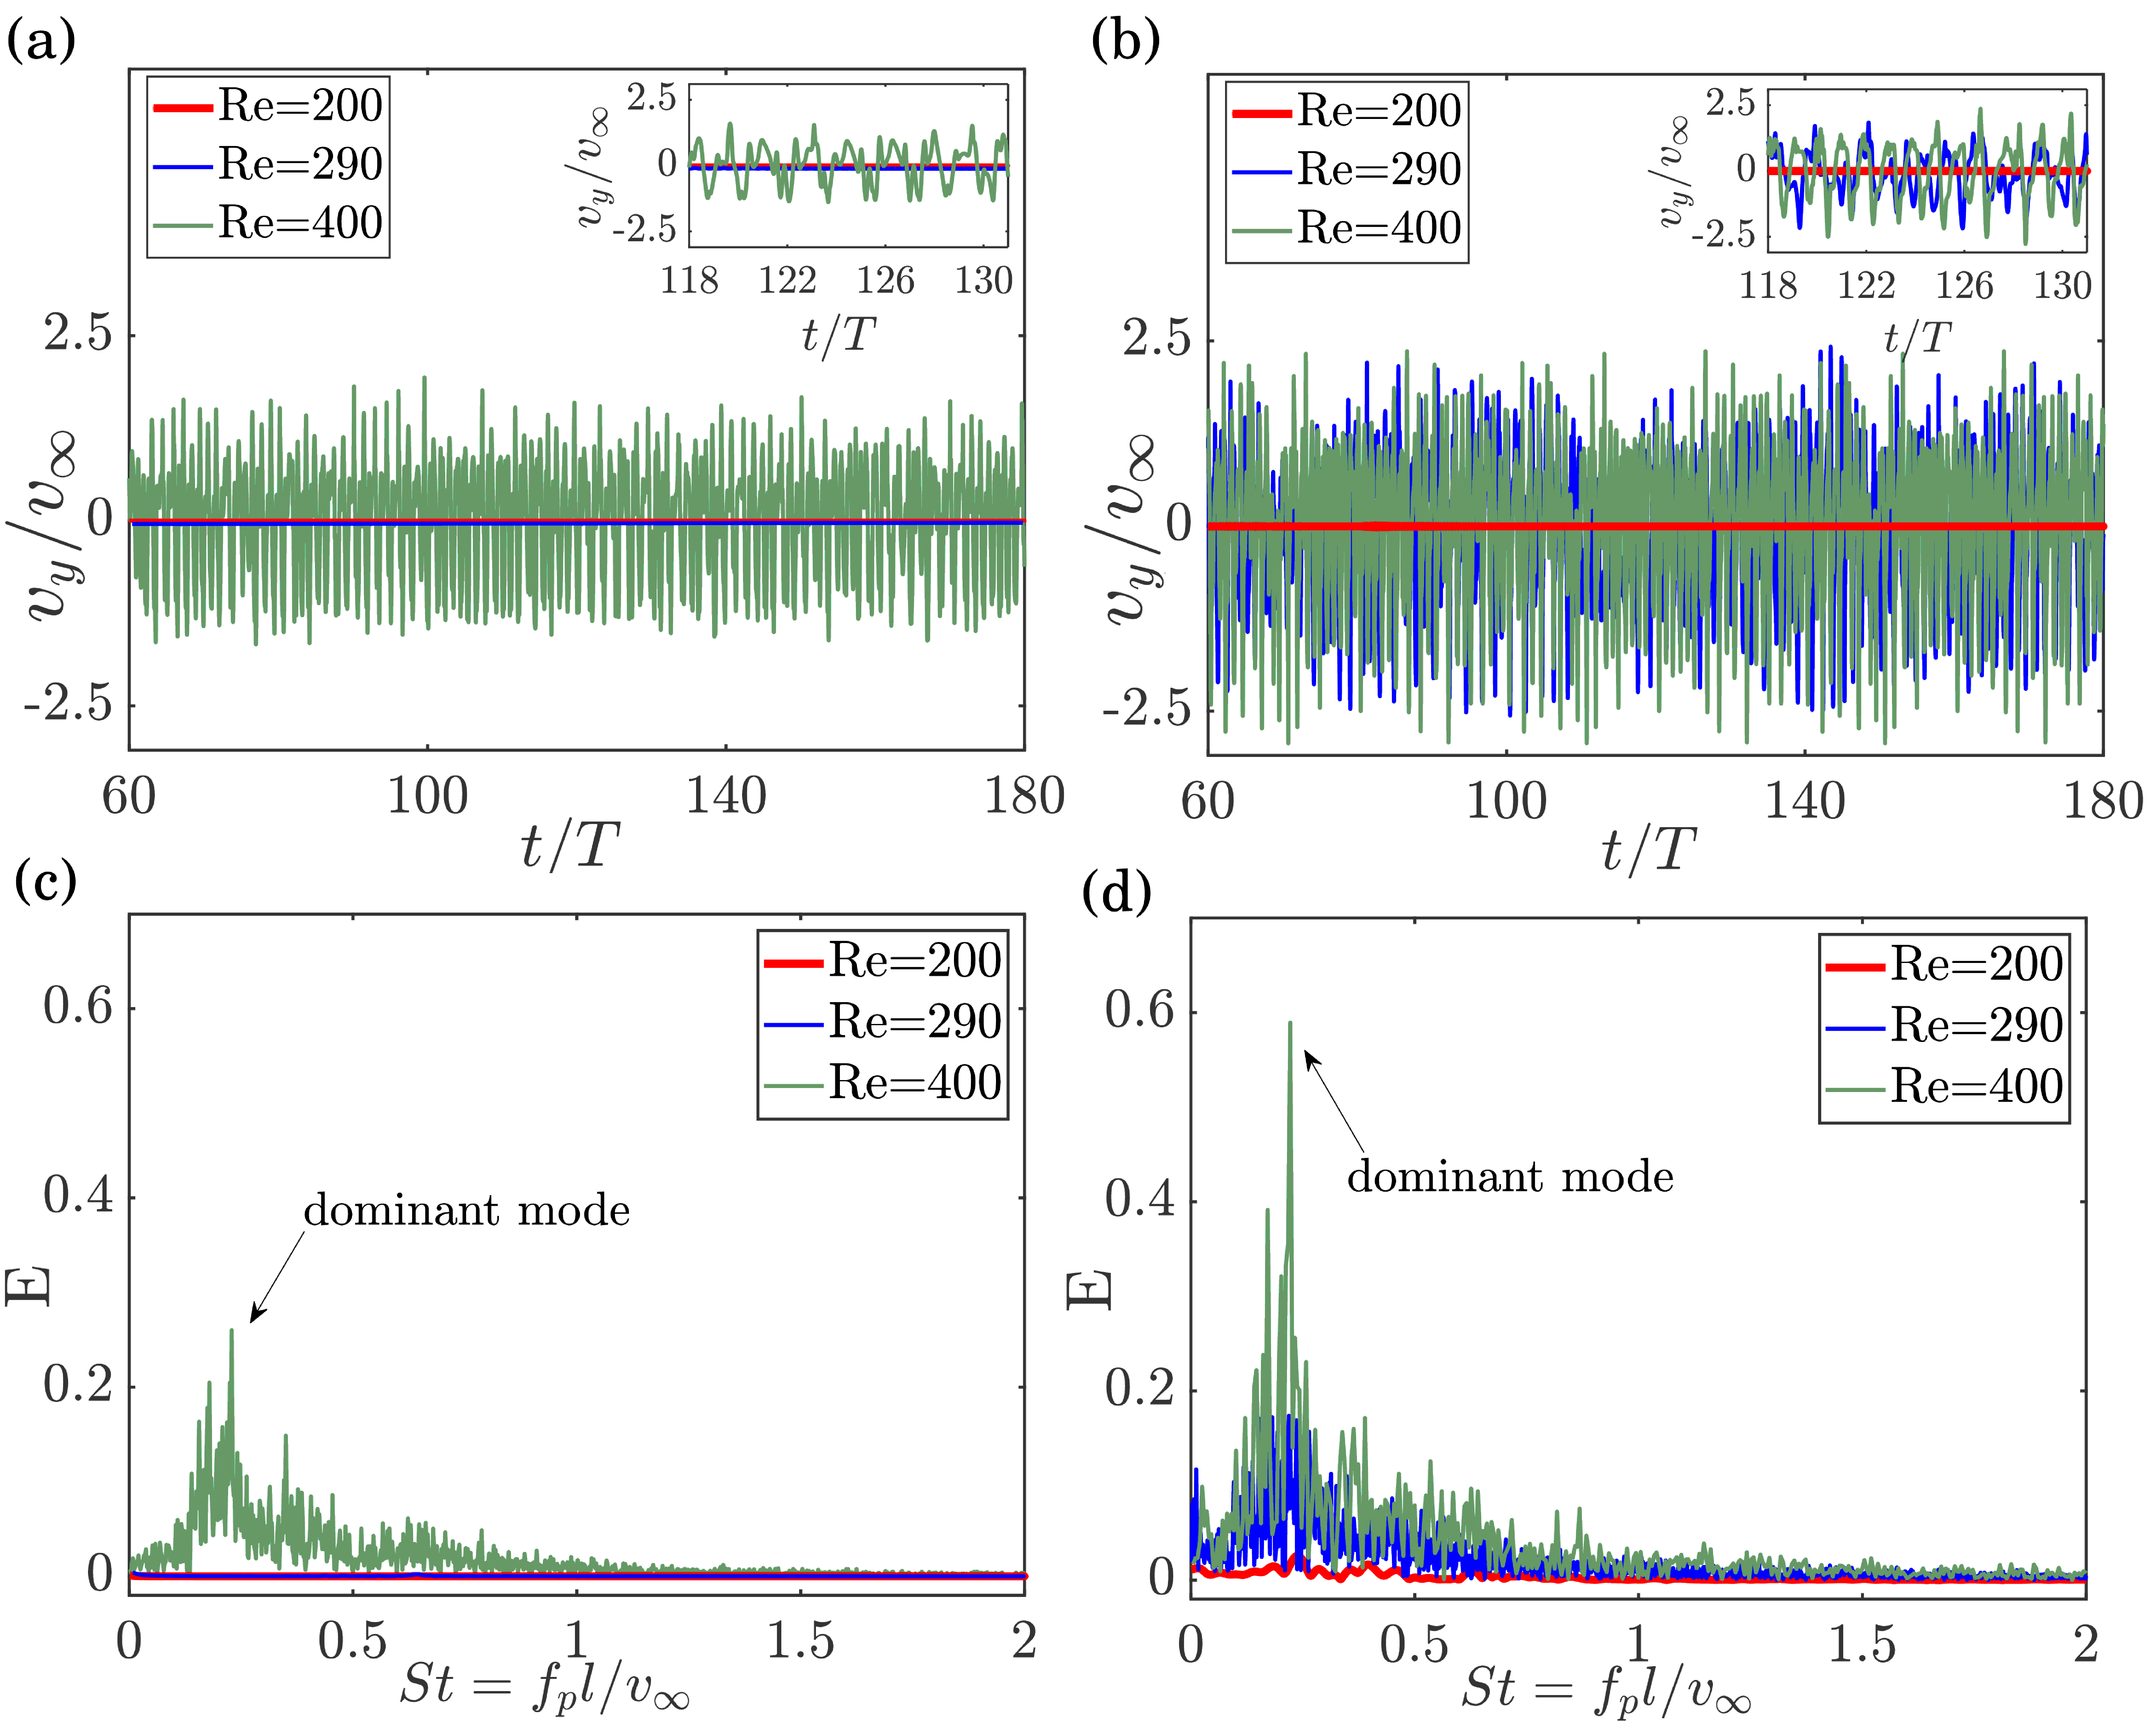
\includegraphics[width=1\linewidth]{Fig12.pdf} 
		\end{minipage} 
		\caption{Cross-wise velocity vs. time measured at point {\fontfamily{phv}\normalsize{X}}$(x=7h,y=0)$ in the downstream for: (a) a single plate case, and (b) a double plate case with $d/h=2$. Spectral energy $E$ vs. Strouhal number ($St$) shown in panels c (for a single plate case) and d (for a double plate case with $d/h=2$). Insets for zoom-up on crosswise velocity time series. Note, the velocity signal for single plate case is $\approx0$ for both $Re=200$ and $Re=290$.}
		\label{fig:t_vs_vy}
		
	\end{figure} 
	
	
	\begin{figure}
		\begin{minipage}[c]{1\linewidth}
			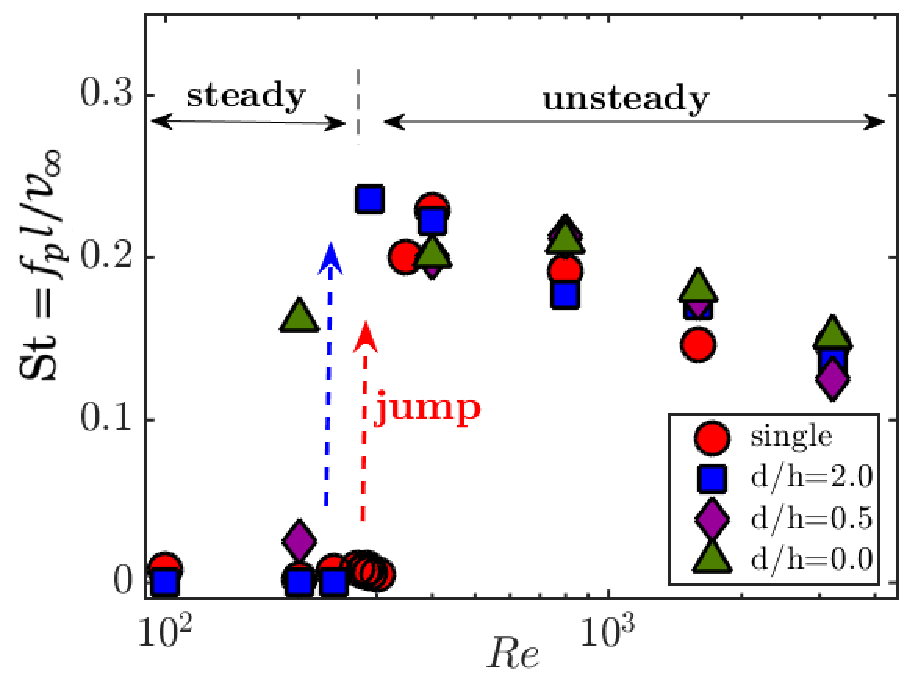
\includegraphics[width=0.90\linewidth]{Fig13.pdf} 
		\end{minipage} 
		\caption{Inlet flow Reynolds number ($Re$) vs. the Strouhal number ($St=f_pl/{v_{\infty}}$). Symbols are circles (single plate), squares ($d/h=2$), diamonds ($d/h=0.5$) and triangles ($d/h=0$).}
		\label{fig:Re_vs_St}
	\end{figure}
	
	It is well known that flow over bluff bodies at high $Re$ leads to vortex shedding in the downstream side~\cite{Sreenivasan1987}. For example, flow over a circular cylinder is steady up to a critical Reynolds number $(Re_{cr})$ of around $48$. Above which, two rows of staggered vortices develop due to the Hopf bifurcation. Similarly, flow passing over a series of cylinders (both the inline and the staggered arrangement) also showed quite exciting features on the flow bifurcation, see~\cite{Williamson1996, Shelley2011, LeeYou2013, Thompson2014}. Usually, single or multi-point velocity measurements taken in the wake (downstream) can reveal the flow instabilities, if present. The point of measurement may range from a distance of few characteristic lengths (for a near-wake behaviour) to a few tens of characteristic lengths (for a far-wake behaviour) in the downstream. In case of flow over cylinders, a wake can be steady if it is measured very near to the cylinder, and can be unsteady if measured in the far field. Both, in experiments and simulations, finding a far-wake behaviour is always challenging due to large information requirement in space and time. It is observed that the near-wake characteristics generally show temporal instabilities, and the far-wake show long wave spatial instabilities~\cite{Saha2003}.
	
	To understand near wake structures developed behind the plates, we have considered a point measurement at a location {\fontfamily{phv}\normalsize{X}} in the flow domain (see figure~\ref{fig:schematic}b). In figure~\ref{fig:t_vs_vy}, the crosswise velocity, $v_y$, is shown as a function of time. The flow meandering due to vortex shedding can be easily recognized from the time series. We observe that the flow bifurcation takes place at $Re_{cr}\approx 370$ in the case of a single plate configuration. In the case of a double plate configuration with $d/h=2$, the flow is steady for $Re<280$ and unsteady for $Re>300$. The critical Reynolds number for $d/h=2$ is found to be $Re_{cr}\approx 290$. With an increase in $Re$, vortices detach from the plates, and the flow becomes unsteady. To bring comparison with the classical plane channel, we briefly explain some of the works which aimed at understanding the flow instabilities in a plane channel. By using linear stability analysis~\citep{orszag_1971} and numerical simulations~\citep{orszag_kells_1980}, $Re\approx 5772$ was reported for a classical plane channel flow. In case of an entry channel flow~\citep{Biau2008}, it was reported that a developing flow has a stabilizing effect on the overall flow, thereby increasing the $Re_{cr}$. The stability characteristics, in general, depends on the amplitude of applied perturbation. Our work is completely different from the classical plane channel flow due to the presence of flexible plates, so a direct comparison is not possible with the aforementioned works. However, it is worthy to notice that the vortices in our work, detach even at $Re<300$, which correspond to an early flow instabilities. In figures~\ref{fig:t_vs_vy}c and d, power spectra of the crosswise velocity signals, calculated using the Fast Fourier Transforms, are shown. In case of a single plate configuration, the flow is unsteady at $Re_{cr}=400$, and therefore, peaks in the energy spectrum are observed. In the case of a double plate configuration, such peaks are observed even at lower Reynolds number, i.e., $Re_{cr}=290$.
	
	
	
	\begin{figure}[b]
		\begin{minipage}[c]{1\linewidth}
			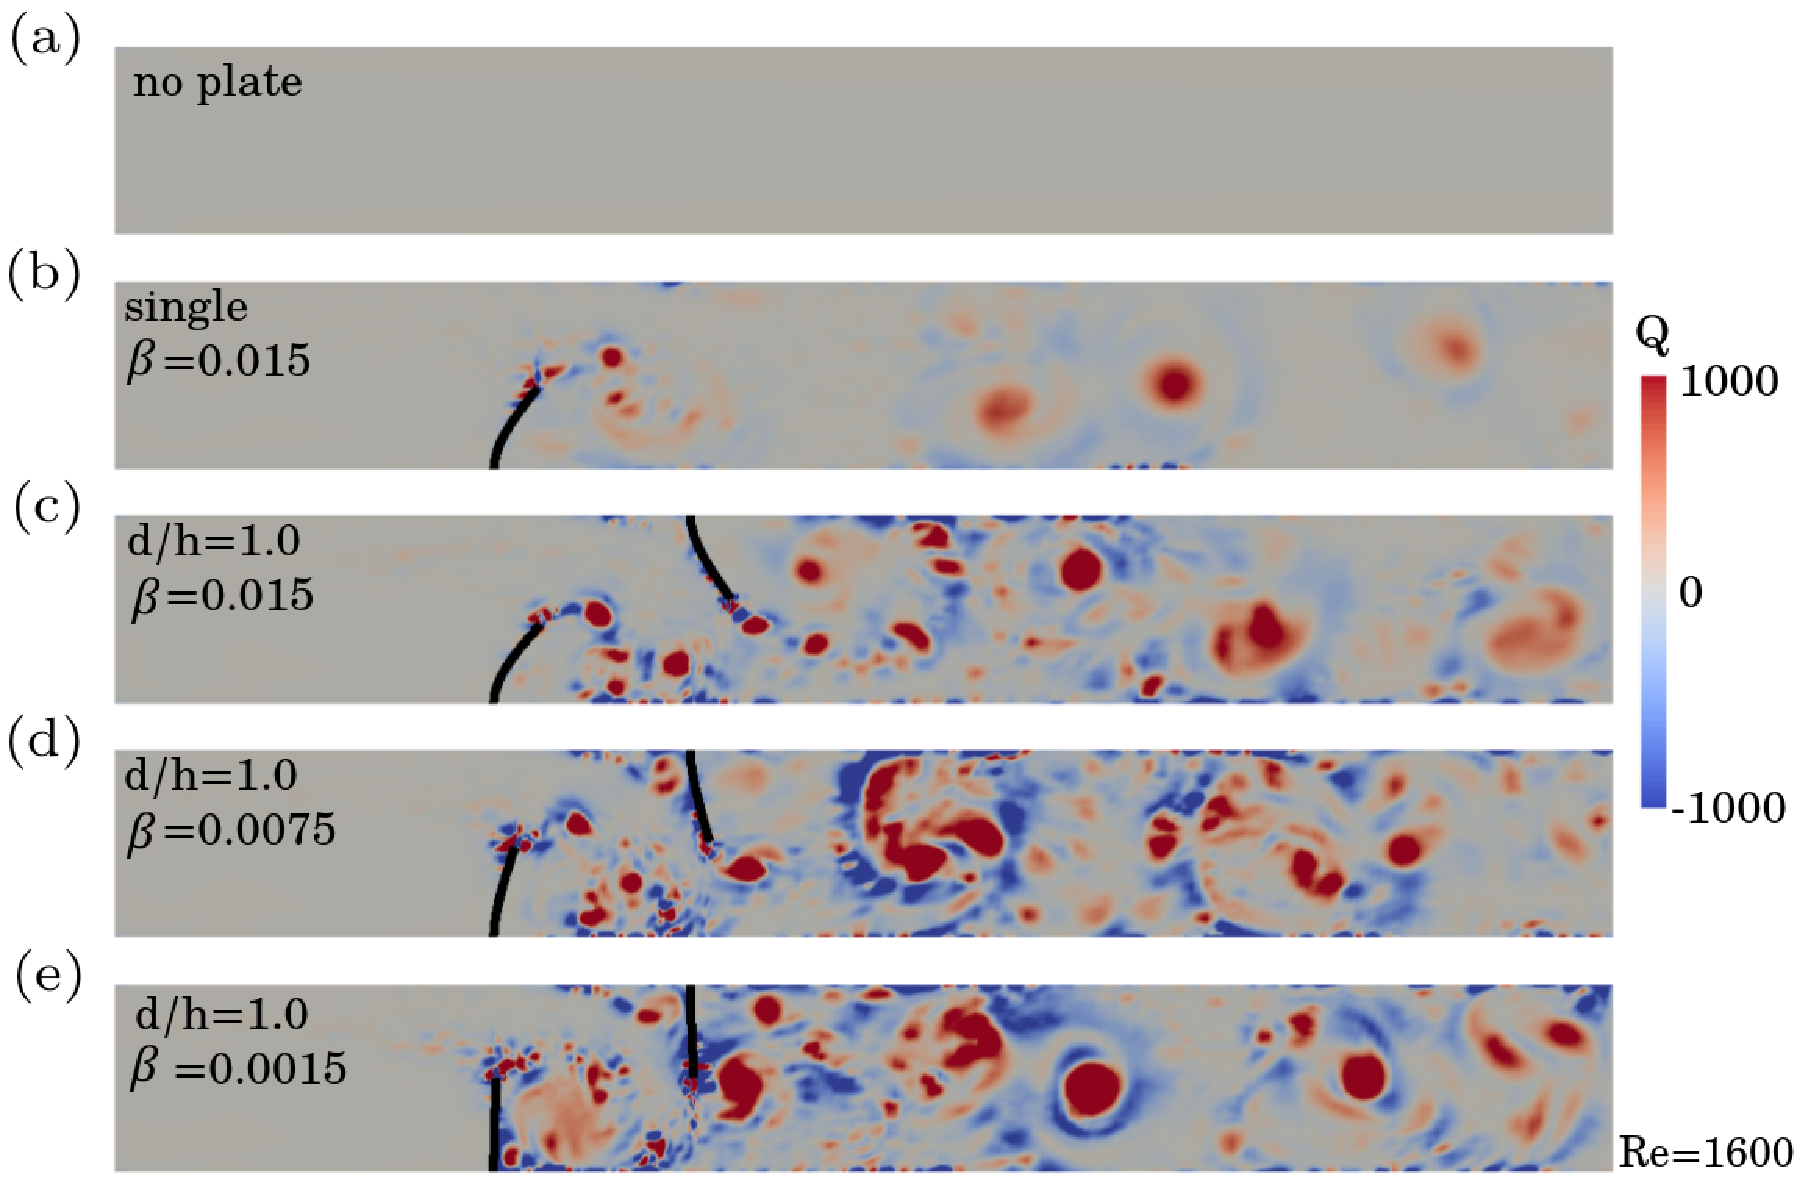
\includegraphics[width=1\linewidth]{Fig14.pdf} 
		\end{minipage} 
		\caption{Q-based instantaneous vortex structures in a channel flow at $Re=1600$: (a) plane channel flow, (b) single plate with $\beta=15\times10^{-3}$, (c) a double plate with the gap $d/h=1$ and $\beta=15\times10^{-3}$, (d) for $d/h=1$ and $\beta=7.5\times10^{-3}$, and (e) for $d/h=1$ and $\beta=1.5\times10^{-3}$. Note, the vortex dominated zones with $Q>0$ and the strain dominated zones with $Q<0$. }
		\label{fig:Re1600_Qvort}
	\end{figure}
	
	
	The dominant flow frequency can be expressed in terms of the Strouhal number, $St=f_p l/v_{\infty}$, which can be interpreted as the resultant crosswise motion generated for a given streamwise flow. Here, $f_p$ is the frequency corresponding to the observed peak in the energy spectrum (or vortex shedding frequency). In figure~\ref{fig:Re_vs_St}, we have identified the steady and unsteady regimes of the flow on $Re$ vs. $St$ plane. In the single plate case, $St\approx 0$ for $Re<370$, and beyond that, we observe a sudden jump in $St$. This jump resembles the classical super-critical Hopf bifurcation, where a steady flow becomes unsteady. In our work, the flexible plates act like catapults and generate strong vortices at the plates' tips. At high $Re$, the vortices move chaotically in the crosswise directions and interact with each other, causing energy to redistribute even at low frequency, and hence a decrease in $St$. In the case of a double plate configuration, $Re_{cr}\approx 290$ for $d/h=2$, and $Re_{cr}\approx 200$ for $d/h=0$. Now, we proceed further to visualize the tip generated vortices. 
	
	\begin{figure*}
		\begin{minipage}[c]{1\linewidth}
			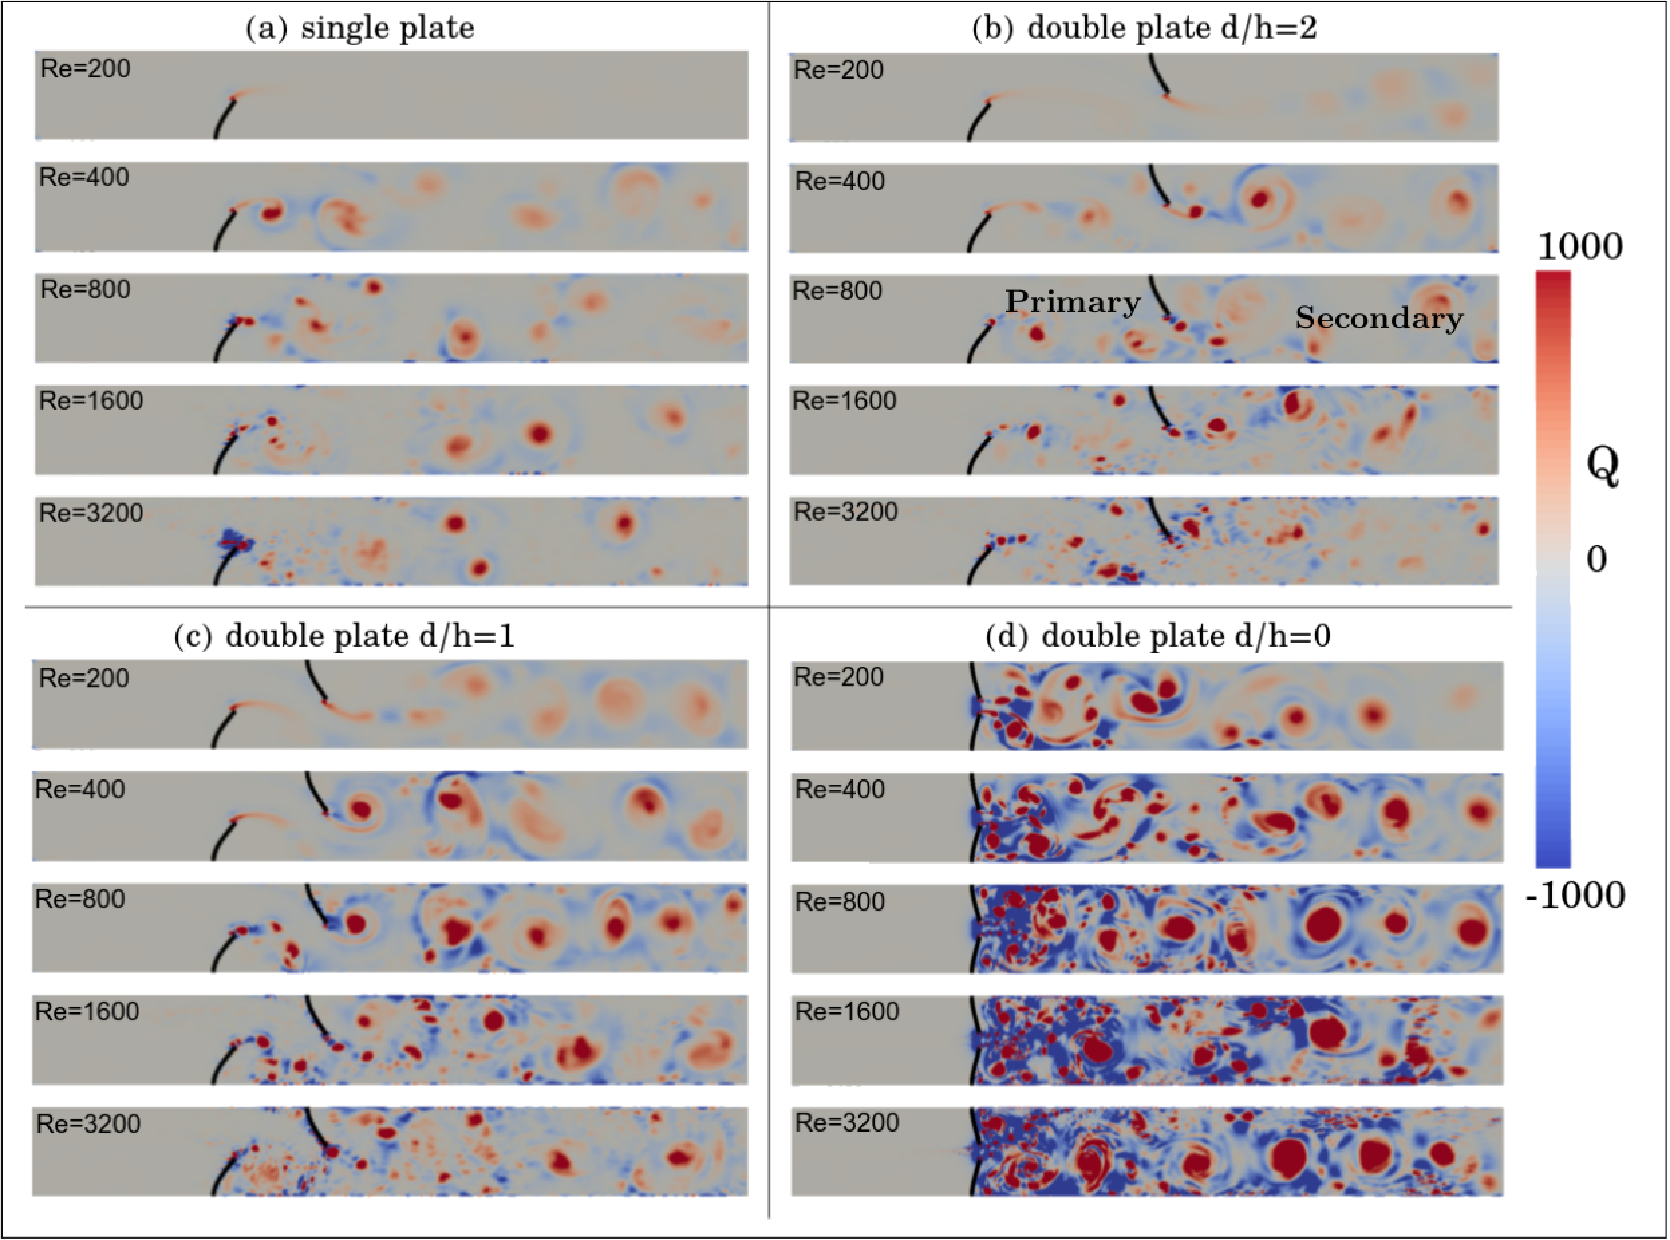
\includegraphics[width=0.9\linewidth]{Fig15.pdf} 
		\end{minipage} 
		\caption{Instantaneous $Q$-based vortex structures for: (a) a single plate, (b) double plates with $d/h=2$, (c) $d/h=1$, and (d) $d/h=0$. In each panel, five simulations are shown with increase in the inlet flow Reynolds number from top to bottom. Note, the vortex dominated zones with $Q>0$ and the strain dominated zones with $Q<0$. See animation 2.}
		\label{fig:Q_double}
	\end{figure*}
	
	
	\subsection{Q-criterion based vortex structures}
	
	In the previous section, information on the flow unsteadiness is explained from a single point measurement. In this section, we have identified the tip detached vortices from the complete spatial-temporal velocity fields. The velocity gradient tensor, $\nabla\mathbf{v}_f$, plays an important role in identifying a flow, whether it is dominated by the rotation, $\mathbf{\boldsymbol{\Omega}}={1\over 2}\left[\nabla\mathbf{v}_f-\nabla\mathbf{v}_f^T\right]$, or by the strain, $\mathbf{S}={1\over 2}\left[\nabla\mathbf{v}_f+\nabla\mathbf{v}_f^T\right]$. In general, the rotational features can be extracted by using any of the following techniques, such as by the vorticity magnitude, the pressure minima, the $\lambda_2$-criteria, or the $Q$-criteria, see~\cite{Hunt1994, Hussain1995, Holmes2012, Rowley2014}. Here, $Q={1\over 2}[|\mathbf{\boldsymbol{\Omega}}|^2-|\mathbf{S}|^2]$ is the second invariant of the velocity gradient tensor. Using $Q$-criterion, strong vortices in the flow (with $Q>0$) can easily be detected during run time calculations without any complex mathematical operations.
	
	
	In figure~\ref{fig:Re1600_Qvort}, $Q$ based instantaneous vortex structures in the plane channel, the single plate configuration, and the double plate configurations are shown. We observe a smooth laminar flow without any vortices in case of the plane channel, as expected. In the case of single and double plate configurations, vortices are generated at the plate's tip. The presence of a second plate generates additional (secondary) vortices in the downstream side, which lead to an increase in mixing level. On increasing the flexural rigidity of the plate (or decrease in $\beta$), we observed an increase in the velocity fluctuations near the plate tips, which disrupt the tip vortices. Two major observations in this regard can be deduced as, (1) the flexible plates generate organized tip detached vortices and outspread (or distribute) them in the flow, and (2) if too rigid plates (or low $\beta$) are used then vortices get disrupted early due to high-frequency tip oscillations. A good mixer design should generate organized vortices in the flow and then should distribute them to mix continuously. So, in that case, a double plate configuration with a moderate $\beta~(=0.015)$ is a better choice in comparison to the case with rigid plates.
	
	\begin{figure*}
		\begin{minipage}[c]{0.85\linewidth}
			\includegraphics[width=1\linewidth]{Fig16.pdf} 
		\end{minipage} 
		\caption{Dominant POD modes in cases of a single plate and double plate configurations: Left panels for $Re=800$, and right panels for $Re=3200$. The dominant spatial mode is represented by velocity vectors and it is color mapped by streamwise velocity fluctuation. Blue (dark) for $-0.02 {v_{\infty}}$ and Red (light) for $0.02{v_{\infty}}$).}
		\label{fig:pod_analysis}
	\end{figure*}
	
	In figure~\ref{fig:Q_double}a, instantaneous vortex structures for a single plate at different $Re$ are shown. The roll strength increases with $Re$ both in terms of the vorticity (by magnitude) and in size. However, for $Re>1600$, high-frequency plate oscillations lead to the disintegration of the vortices at the tips. Indeed at $Re=3200$, the plate tip oscillation frequency is so high that a full vortex roll hardly develops. It is worthy to notice that small scale disturbances propagate in the upstream side of the plate 1 (see animation 2). A separate set of simulations of a long channel of length $10h$, for which the plate 1 is at a distance of $4h$ from the entrance, is also carried out to see the existence of these upstream propagating disturbances. We found that these disturbances are robust and are not any numerical artifact. In figure~\ref{fig:Q_double}b to~\ref{fig:Q_double}d, vortex structures in a double plate configurations are shown. From the figures, it is evident that the plate 2 constraints the primary vortex and significantly promotes a secondary vortex. On decreasing the gap between the plates, many small-scale organized vortices are developed.
	%
	
	
	\subsection{Proper orthogonal decomposition and dominant modes}
	
	
	The time evolution of vortices and their interaction is understood in the previous subsection. To get the time-averaged large scale roll information, we have used the proper orthogonal decomposition technique (POD), which is based on the `Method of Snapshots'~\cite{Holmes2012}. The procedure is as follows, (1) a mean velocity field is calculated from time snapshots, then (2) the instantaneous velocity fields subtracted from the mean field are obtained to get a set of $M$-number of fluctuating velocity fields $\mathbf{v}^{1\, \text{to}\, M}$, and finally, (3) an orthonormal basis set of functions $\mathbf{\Phi}=\sum_{k=1}^{M} c_k\mathbf{v}^k$ are constructed, where the coefficients $c_k$ satisfies the eigenvalue problem 
	$[{1\over M}\mathbf{v}^i\cdot\mathbf{v}^j-\lambda \delta_{ij}]\mathbf{c}=\mathbf{0}$. Here, $\lambda$ is the eigenvalue, $\delta_{ij}$ is the Kronecker delta, and $\mathbf{0}$ is the null vector. The constructed basis has a property in extremizing the inner product of $\mathbf{v}$ and $\mathbf{\Phi}$, i.e., maximize ${1\over{|\mathbf{\Phi}\cdot\mathbf{\Phi}|^2}}\langle{|\mathbf{v}\cdot\mathbf{\Phi}|^2}\rangle$, where $\cdot$ is the inner product, and $\langle\rangle$ is the ensemble average. The relative energy of any principle orthonormal mode is given by $E_k=\lambda_k/{\sum_k \lambda_k}$. By sorting the eigenmodes in the increasing order of energy content, we have isolated the dominant energy mode. 
	
	
	In figure~\ref{fig:pod_analysis}, the dominant POD modes obtained for the single and the double plate configurations are shown. In the case of a single plate configuration, the dominant energy mode is a pattern of four or five rolls placed next to each other, which spans over a length of $6h$, in the streamwise direction. The strength of these rolls increases with an increase in $Re$ (see the streamwise velocity fluctuation contours). In the double plate case, the number of rolls and their span extent depends on the plate 2. Note, the vortices are absent in the upstream direction of the plate 2. On decreasing the plates' gap from $d/h=2$ to $d/h=0$, many rolls are observed in the downstream. Notably, the modes are always found next to the plate 2, but not at the plate 1, indicating that the secondary vortices are strong and the primary vortices are suppressed. Indeed, the flow instabilities discovered on $Re$ vs. $St$ plane are due to these secondary vortices.
	
	\section{Energy dissipation rates}
	
	
	\begin{figure}
		\begin{minipage}[c]{1\linewidth}
			\includegraphics[width=0.85\linewidth]{Fig17.pdf} 
		\end{minipage} 
		\caption{(a) Volume and time-averaged energy dissipation vs. inlet flow $Re$, and (b) relative energy dissipation in a double plate case when compared to a single plate case vs. $Re$. Closed (or filled) symbols are for $\beta=1.5\times 10^{-2}$, and open symbols (or unfilled) for $\beta=1.5\times 10^{-3}$. As a grid convergence check an additional simulation is carried out with a fine mesh resolution for $d/h=2$ (marked as \textcolor{magenta}{ \fontfamily{phv}\large{X}}). In the inset, the normalized energy dissipation vs. $\beta$ shown for $Re=1600$. Note, $\overline{\epsilon}_S$ is the volume and time-averaged energy dissipation in case of a single plate anchored in a channel flow.}
		\label{fig:ener_1a}
	\end{figure}
	
	
	In three-dimensional turbulent flows, energy is fed at the large scales, and it cascades downwards by dissipating at the small scales, namely, the Kolmogorov micro-scale, $\eta=(\nu^3/\overline{\epsilon})^{1/4}$. Here, $\epsilon= {\nu}\int_{\volume}\, |\nabla\mathbf{v}_f|^2\, d\volume$ is the volume-averaged energy dissipation, where $\volume$ is the volume average considered. In the case of a 2D flow, large scale generation is possible from the smaller scales through the inverse cascade mechanism~\citep{Boffetta2012, Mishra2015}. For both 2D and 3D flow fields, the `stir' created in the flow by different scales of motion, helps in re-distributing the scalar fields. Eventually, all the gradients smear at the small scales by the molecular diffusion; thus, thorough mixing takes place. The flow instabilities helps in increasing the local flow fluctuations and may lead to an increase in the mixing rate. To understand the flow scale separation, we have computed volume and time-averaged energy dissipation in the channel for the single and the double plate configurations. 
	
	
	
	In figure~\ref{fig:ener_1a}, the volume and time-averaged energy dissipation ($\overline{\epsilon}$) as a function of $Re$ is shown. We can observe an increase in $Re$ corresponds to an increase in the energy dissipation. The dissipation level can be increased up to two orders of magnitude by decreasing the plates' gap from $d/h=2$ to $d/h=0$. We have compared the energy dissipation in a double plate configuration with respect to the single plate as, ${\overline{\epsilon}/\overline{\epsilon}_S}$, as shown in figure~\ref{fig:ener_1a}b. Here, $\overline{\epsilon}_S$ is the time and volume averaged dissipation in the single plate case. The dissipation level in a double plate case is always higher than that in a single plate case. Additionally, to understand the role played by the flexural rigidity of the plate, we have decreased the parameter $\beta$ from $1.5 \times 10^{-2}$ to $1.5\times 10^{-3}$ (see the open symbols in figure~\ref{fig:ener_1a}) and observed an increase in the energy dissipation.
	
	
	
	\begin{figure}
		\begin{minipage}[c]{1\linewidth}
			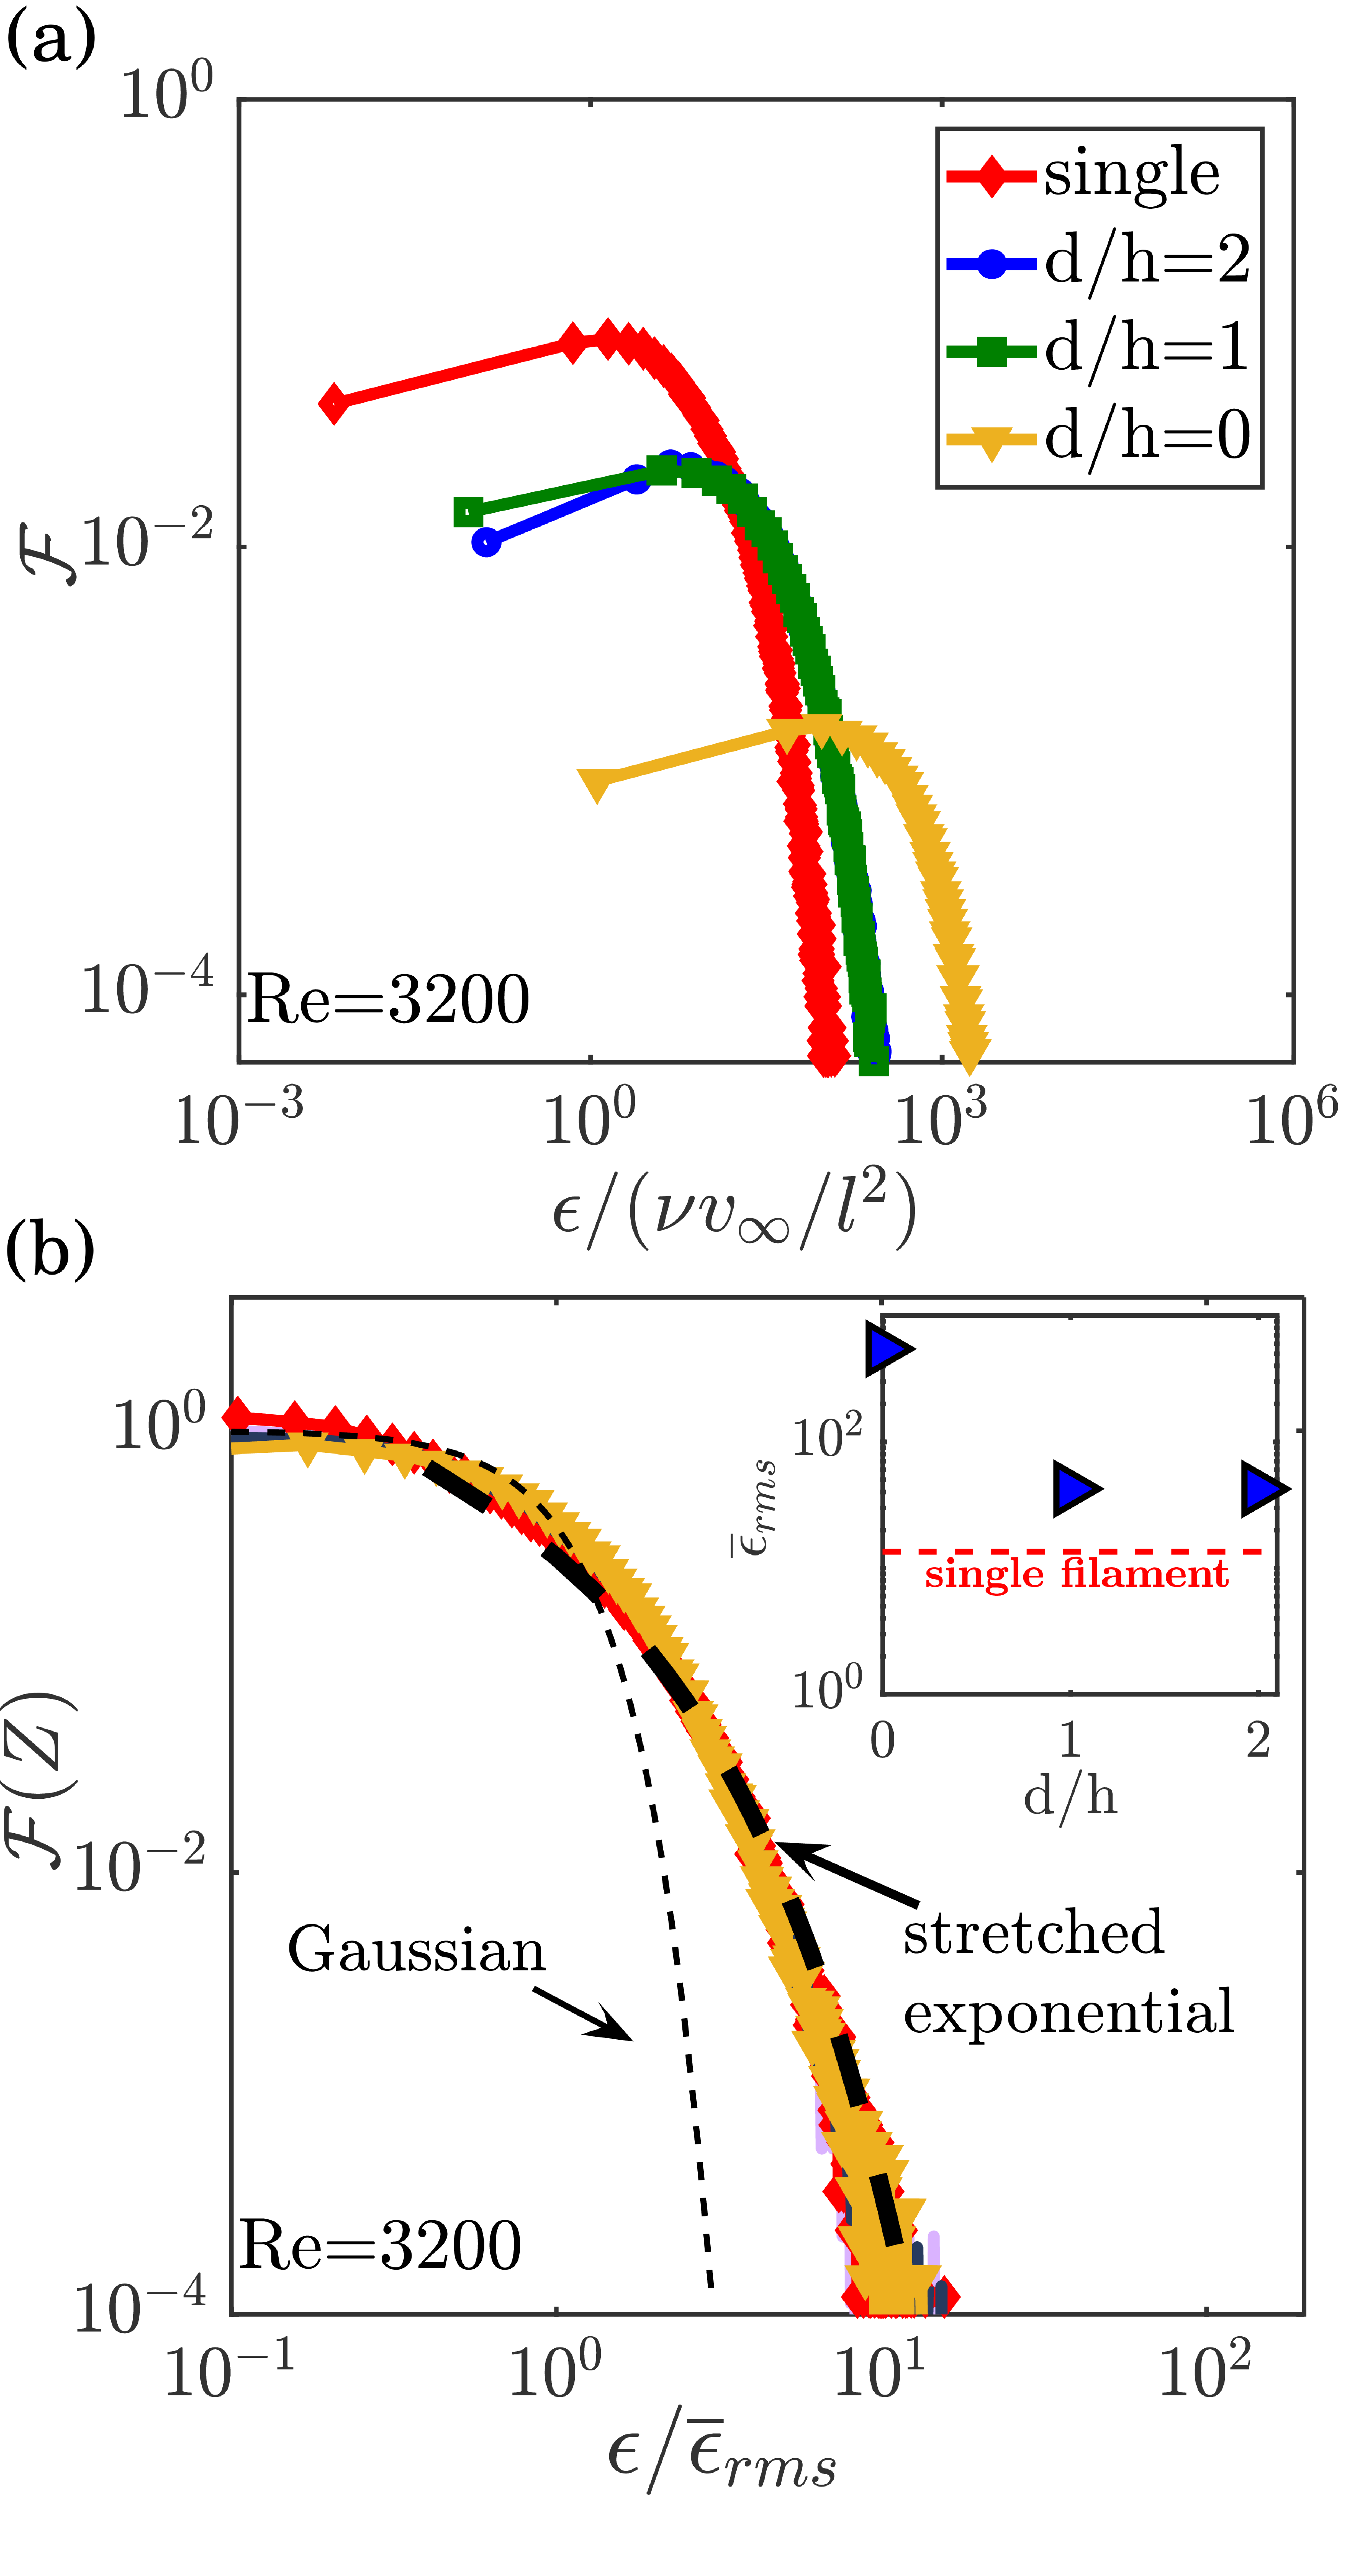
\includegraphics[width=0.90\linewidth]{Fig18.pdf} 
			% 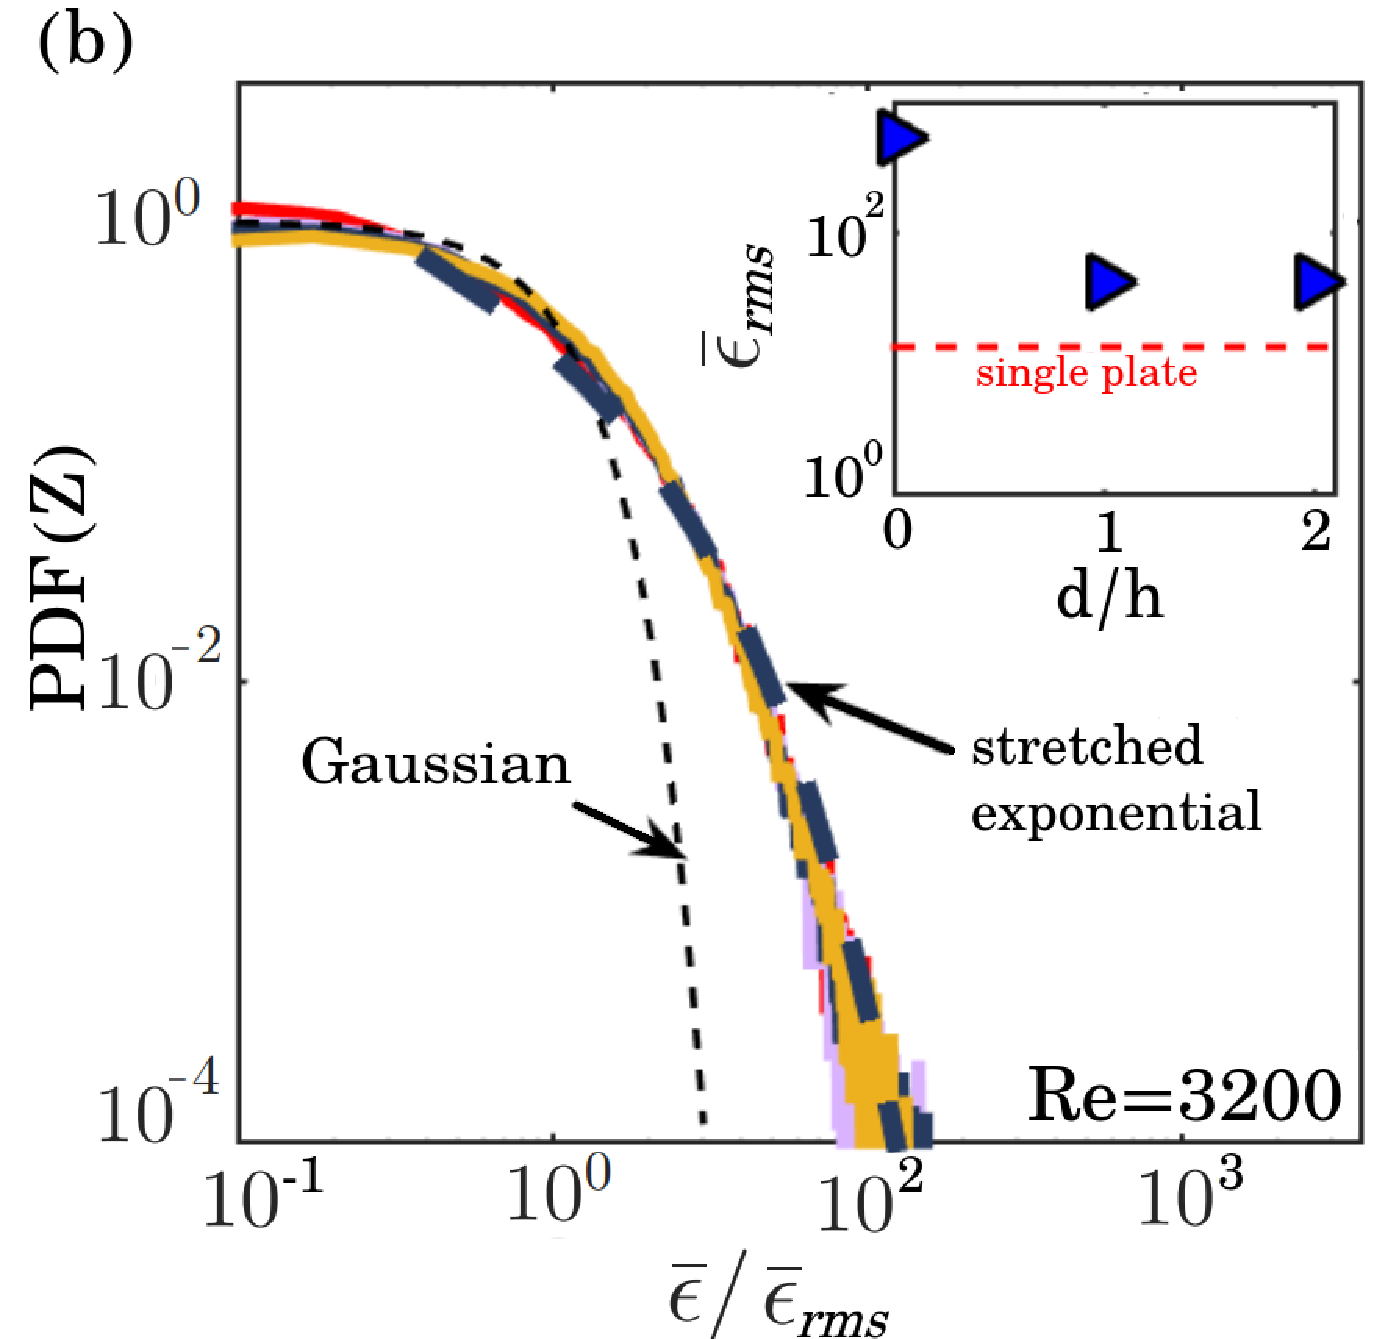
\includegraphics[width=0.78\linewidth]{Fig18b.pdf} 
		\end{minipage} 
		\caption{(a) Probability density function ($\mathcal{F}$) of the kinetic energy dissipation, and (b) $\mathcal{F}$ vs. $\epsilon/\overline{\epsilon}_{rms}$. Normal Gaussian curve in thin dashes and a stretched exponential in thick dashes are shown. Inset for $\overline{\epsilon}_{rms}$ as a function of plate gap $d/h$. Simulations are for $Re=3200$ and data statistics taken at the channel core in Region A.}
		\label{fig:doublefil_Re3200}
	\end{figure}
	
	
	\begin{figure}
		\begin{minipage}[c]{1\linewidth}
			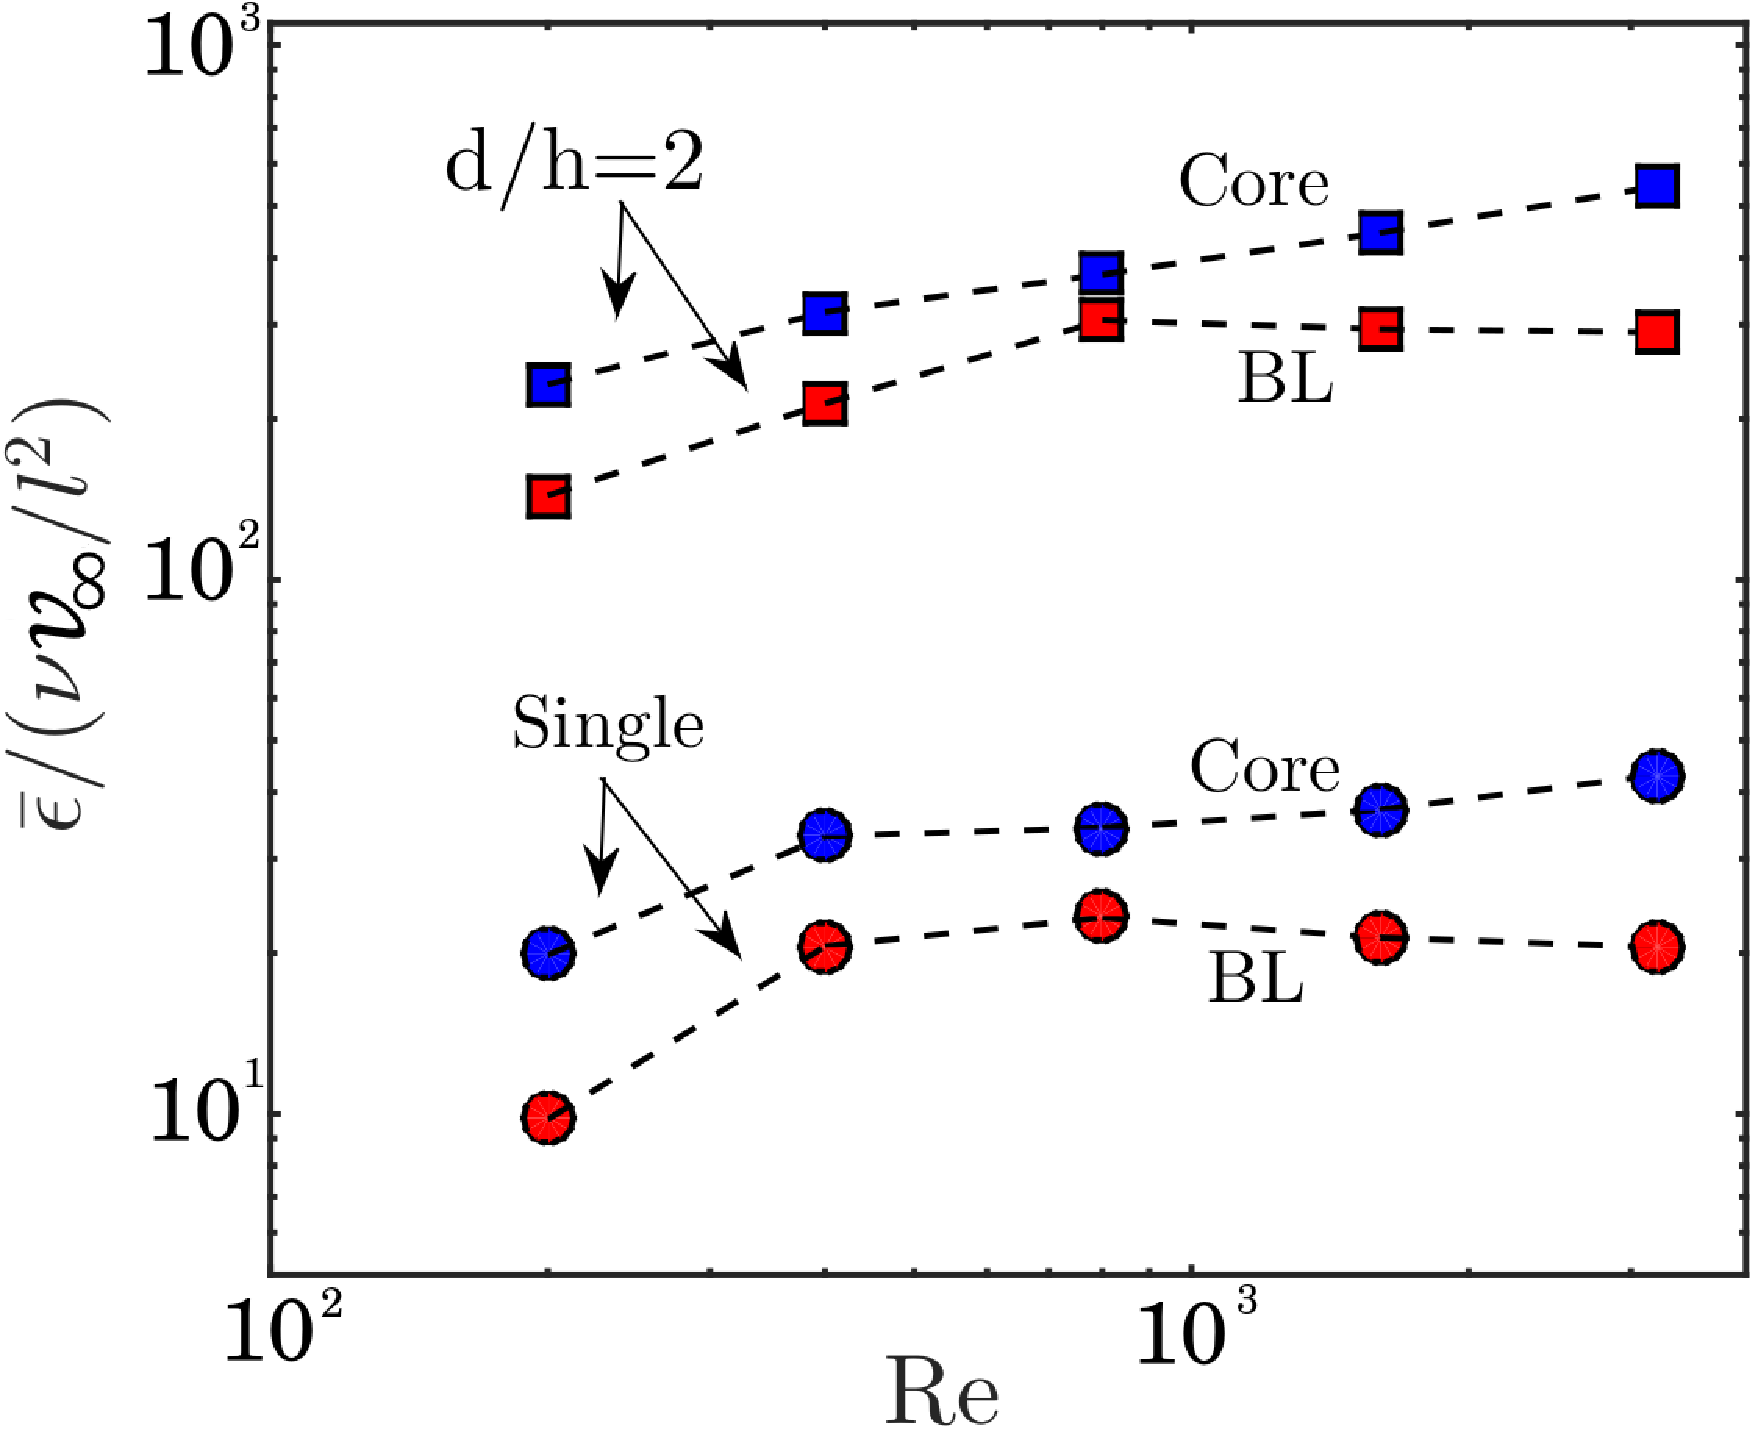
\includegraphics[width=0.95\linewidth]{Fig19.pdf} 
		\end{minipage} 
		\caption{Volume and time-averaged kinetic energy dissipation vs. $Re$: at the channel core (or bulk) zone and in boundary layers. Symbols: circles for a single plate channel flow and squares for a double plate channel with gap $d/h=2$.}
		\label{fig:core_BL_vs_Re} 
	\end{figure}
	
	
	\begin{figure}
		\begin{minipage}[c]{1\linewidth}
			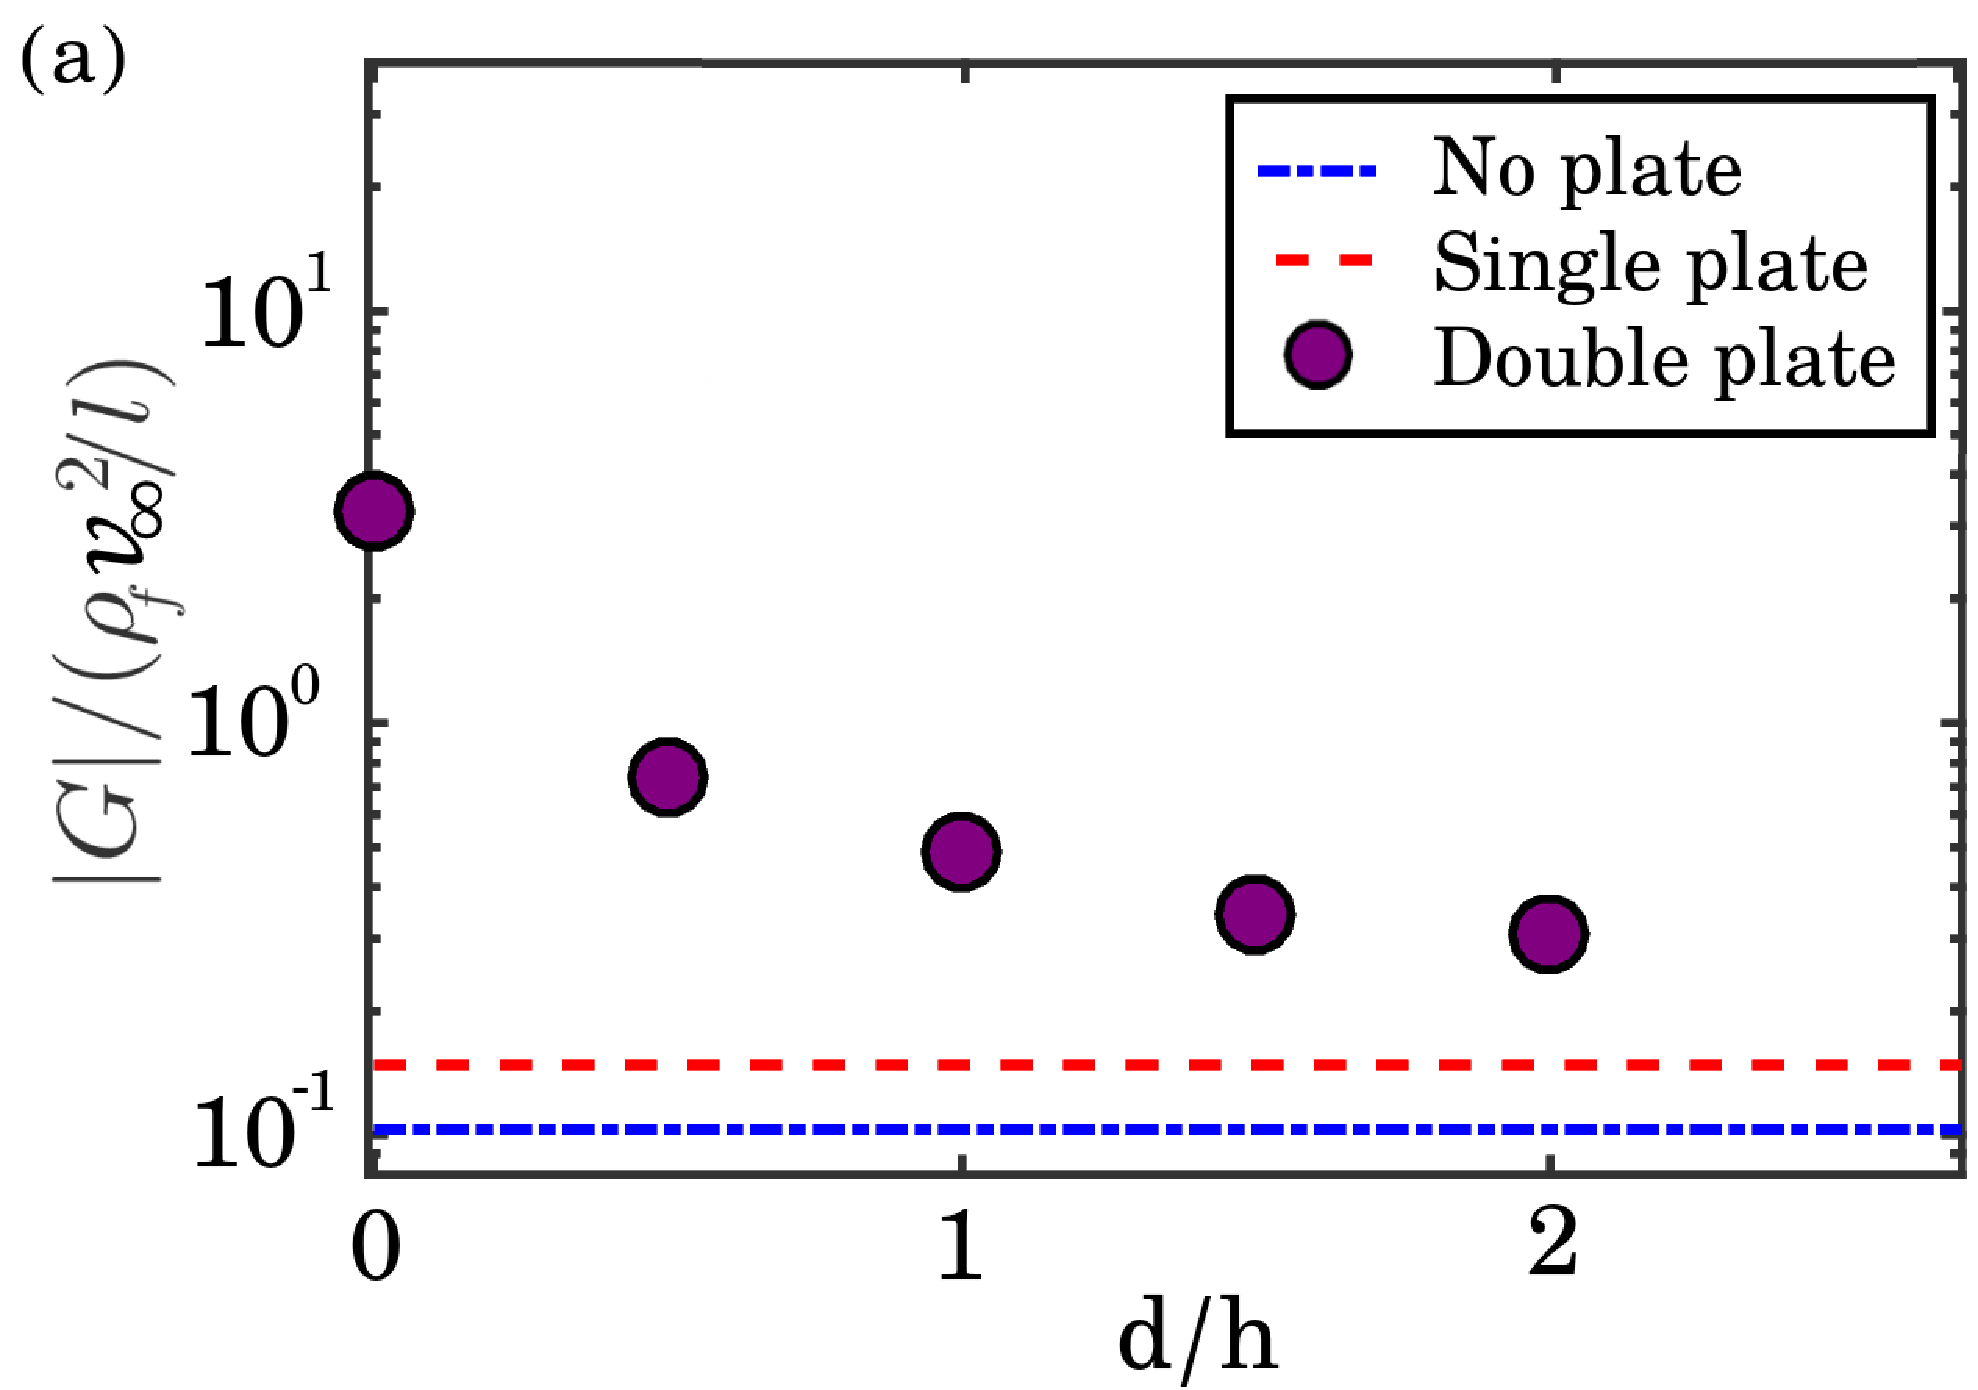
\includegraphics[width=0.95\linewidth]{Fig20a.pdf} \\
			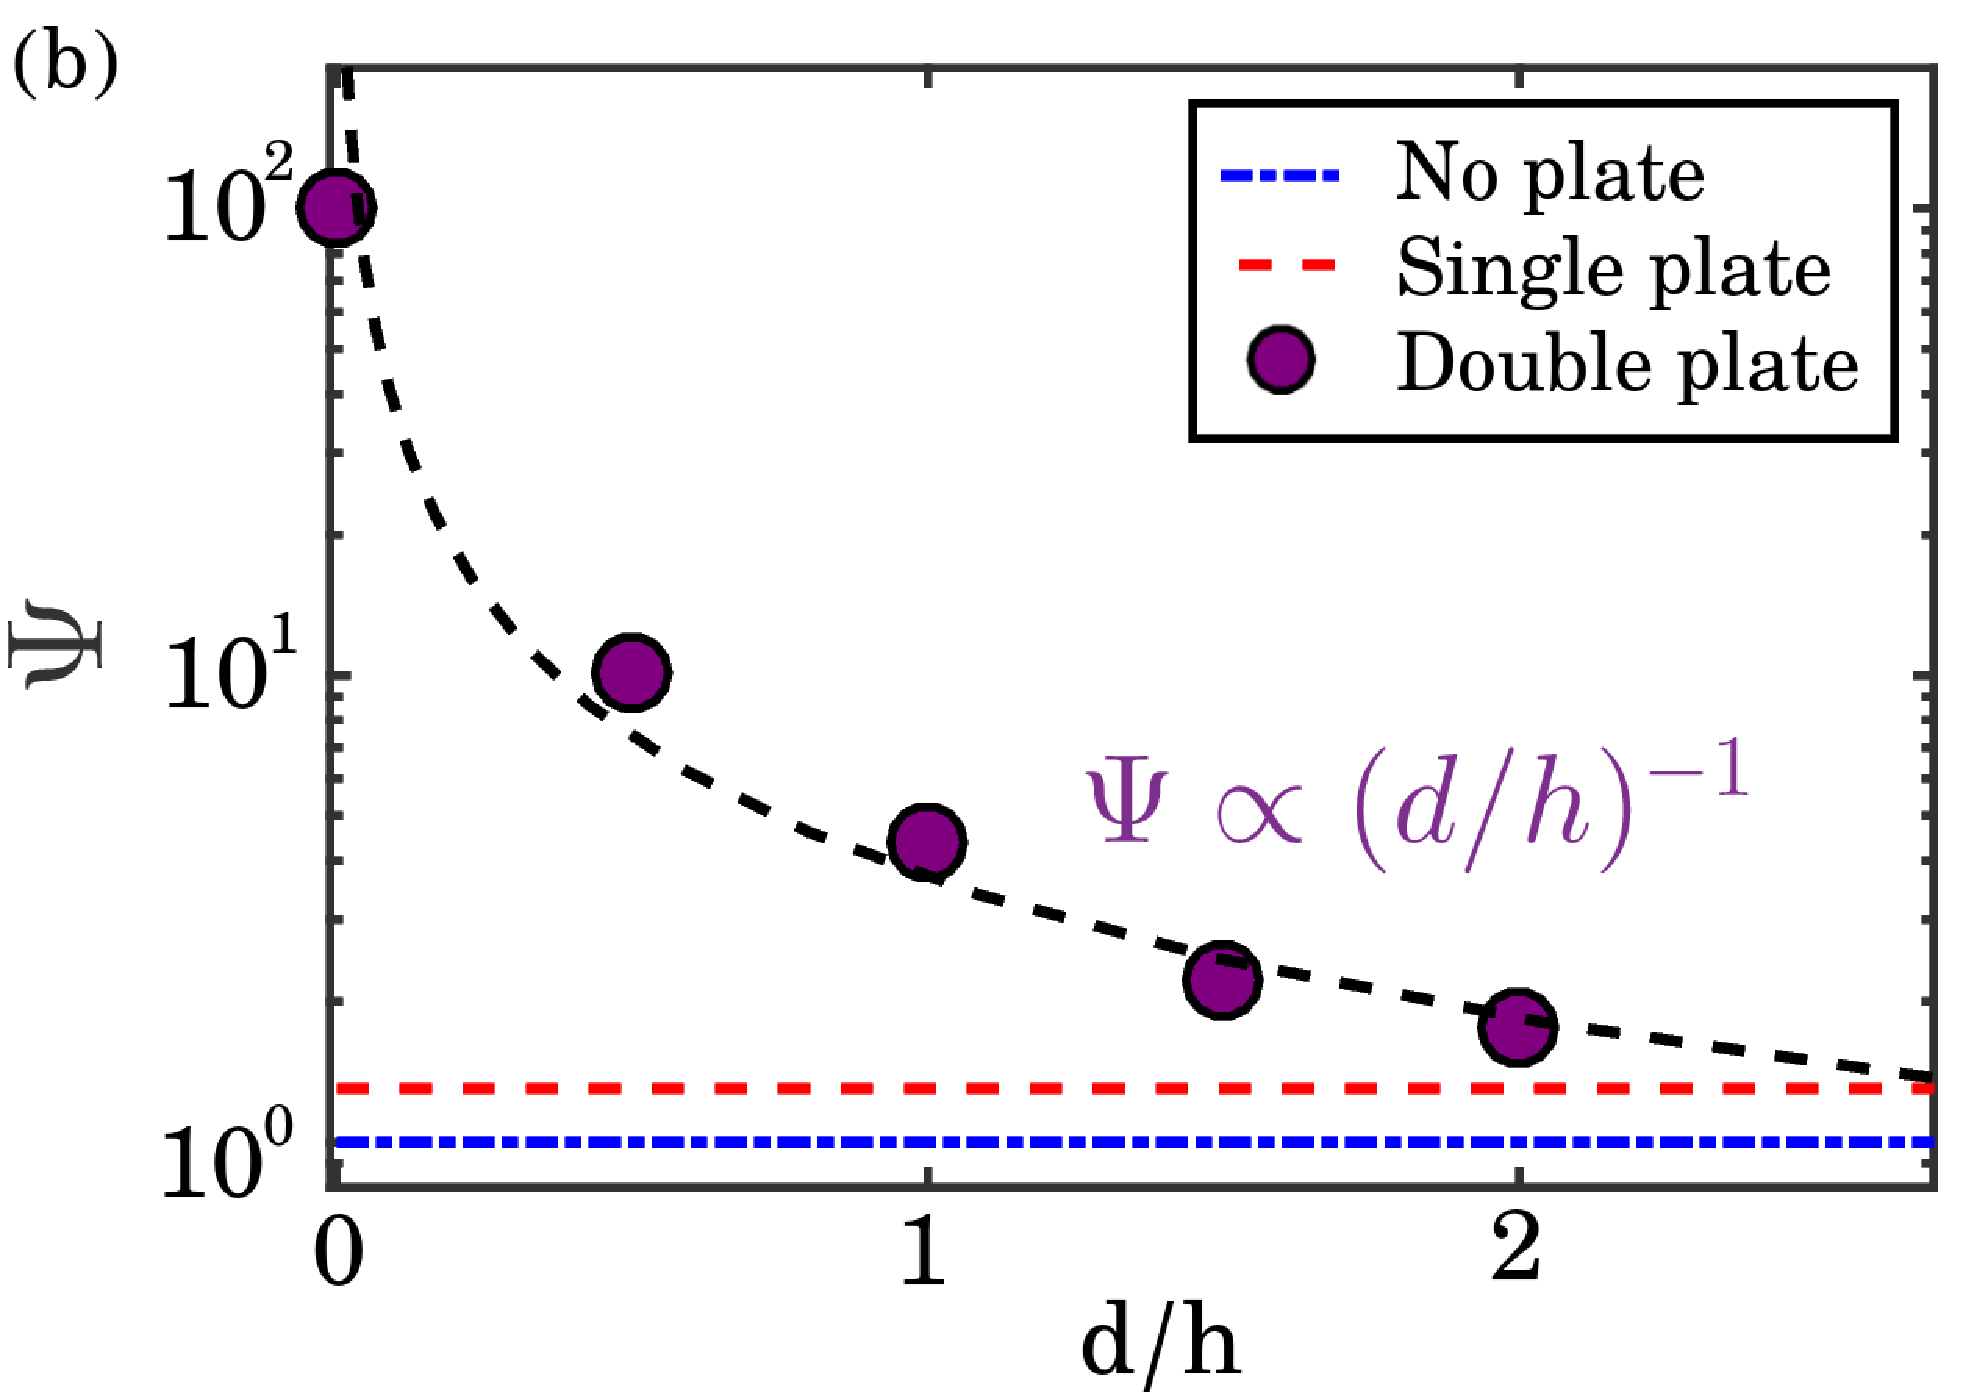
\includegraphics[width=0.95\linewidth]{Fig20b.pdf} 
		\end{minipage} 
		\caption{(a) pressure gradient (loss) vs. $d/h$, and (b) $\Psi$ vs. $d/h$. Channel flow simulations without any anchored plates (dash-dot line), with a single anchored plate (dash line) and a double plate configuration (circles). Note, $\Psi=1$ for a plane channel flow without anchored plates, and $\Psi=1.3$ for a single plate channel flow. Best fit (dashed line through the circles) suggests $\Psi\propto (d/h)^{-1}$ for a double plate configuration. Simulations are for $Re=1600$.}
		\label{fig:core_BL_vs_Re2} 
	\end{figure} 
	
	
	The wide distribution of scales in a mixing process can be understood from the probability density function ($\mathcal{F}$) of the energy dissipation. In phenomenological turbulence models, the dissipation is usually assumed to exhibit log-normal distribution, and any deviation from this behaviour indicates intermittency in the turbulence. The recent studies~\cite{lohsearfm,LohseGrossmann1993} suggest that the dissipation statistics follow the stretched-tail distribution of the form $\mathcal{F}(Z)= {a\over{\sqrt{Z}}}e^{-pZ^{q}}$, where $Z = {\epsilon/ {\overline{\epsilon}_{rms}}}$ is the normalized dissipation, and $a$, $p$, $q$ are the fit parameters and $\overline{\epsilon}_{rms}$ is the root mean square value of the energy dissipation. For $q=2$, $\mathcal{F}$ shape corresponds to the Gaussian curve, and for $q=1$, $\mathcal{F}$ shows a simple exponential curve. In figure~\ref{fig:doublefil_Re3200}a, $\mathcal{F}$ of the energy dissipation for the single and the double plate configurations are shown. The dissipation statistics are taken at the channel core in region A, see figure \ref{fig:schematic}b, where intense mixing is observed. The computed $\mathcal{F}$ show long tails and deviate from the normal Gaussian. The mean dissipation level also increases by decreasing the plates' gap. To distinguish the intermittent events, we have shown the $\mathcal{F}$ of the normalized dissipation, ${\epsilon}/\overline{\epsilon}_{rms}$ in figure~\ref{fig:doublefil_Re3200}b. For ${\epsilon}<\overline{\epsilon}_{rms}$, the $\mathcal{F}$ follow the normal Gaussian curve. However, the least-likely dissipation events at the $\mathcal{F}$ tails (which are very intense events with ${\epsilon}\approx 10\overline{\epsilon}_{rms}$), follow the stretched exponential curve with the parameters $p=0.89$ and $q=0.86$. It is interesting to note that the fit parameters obtained in our simulations closely match with the values reported in a completely different configuration such as the Rayleigh-Taylor turbulence, see~\cite{ZhouJiang2013}. We bring this comparison to indicate that the small-scale behaviour may be the same and universal, independent of the driving conditions.
	
	The total energy dissipated in the channel can be evaluated as the sum of the energy dissipated by the wall shear and by the vigorous fluctuations in the core. An independent analysis of both the near-wall and the core (bulk) regions can identify the specific transport mechanism. To separate these effects, we have identified both the boundary layers and the core zone in the region A, as shown in figure~\ref{fig:schematic}b. In this region, the flow remains unaffected from the plates' immediate impact and contains the advecting large-scale and small-scale vortices. We have compared the dissipated energy contribution in the core zone with that of the boundary layer zone, in figure~\ref{fig:core_BL_vs_Re}, where the weighted volume and time-averaged energy dissipations as a function of $Re$ are shown. We can observe that the dissipation in the core zone is higher than in the boundary layer zone by more than $60\%$. Both the core and the wall shear dissipation increase, if the plate 2 is present.
	
	
	The increased energy dissipation is observed at the cost of pressure loss in the channel. In the following discussion, we quantitatively investigate the same. In a steady laminar channel flow under fully developed conditions, the balance between the viscous and the pressure force leads to the parabolic velocity profile, $\mathbf{v}_f(y)=(G/2\rho_f\nu)y(y-h)$, where the pressure gradient, G=${-dP\over dx}={-\Delta P\over L}$ is constant. Usually, the pressure loss $\Delta P=P_{outlet}-P_{inlet}$ takes place to overcome the drag, and is measured as the difference between the exit and the entrance pressures. The rate of work done can be estimated as $\mathscr{P}=\int_{A}\mathbf{v}_f\cdot \Delta P d\mathbf{S}=-{G^2Lh^3b/(12\rho\nu)}$, where $\mathbf{S}$ is the surface area of the channel's control volume. At steady-state, the dissipated power per unit mass of the fluid is calculated as $\mathscr{P}/(\rho_f Lhb) =-G^2h^2/(12\rho_f^2\nu) \equiv\overline{\epsilon}$, which indicates that an increase in pressure loss corresponds to an increase in overall energy dissipation. In figure~\ref{fig:core_BL_vs_Re2}a, the loss in pressure gradient for different configurations is compared. The pressure loss increases by decreasing the plates' gap. The observed pressure loss for $d/h=0$ is nearly 30 times to that of the loss observed in a plane channel. Note that, in case of a steady plane channel flow, $G^2/\overline{\epsilon}=$ constant. Indeed, this ratio identifies an unwanted pressure loss incurred for the desired mixing. To understand the increase in pressure loss due to the presence of flexible plates, we have calculated $\Psi={\left[{G^2/ \overline{\epsilon}}\right]_{plate} \over \left[{G^2/\overline{\epsilon}}\right]_{laminar}}$. For a steady plane channel flow, $\Psi=1$, and the pressure loss observed is completely due to the viscous shear at the walls. For $\Psi> 1$, the dissipation consists of both the core and the boundary layer contributions. In figure~\ref{fig:core_BL_vs_Re2}b, $\Psi$ vs. $d/h$ is shown. We found a relation, $\Psi\propto (d/h)^{-1}$ based on the best fit using the least squares method. For a wide gap between the plates, the normalized pressure loss approaches a value equal to the single plate case. We observed $\Psi\approx1.3$ for $d=3h$, on further extrapolating the curve. Note, the proposed scaling of the pressure loss may depend on the number of plates and other factors too. We request the scientific community to check the robustness of the proposed scaling law for small-scale mixing applications. Any further investigation like increase in the number of plates, their spatial orientation, variation in flexibility ratios, and additional three-dimensional effects shall indeed provide a great insight to design efficient mixing devices and would be of future scope. 
	
	\section{Summary and Conclusions}
	
	Two-dimensional numerical simulations based on the fluid-structure-interaction framework have been used to characterize the flow past one or two flexible plates anchored to opposite walls of a channel. The inlet flow Reynolds number ($Re$) in the channel is varied in the range $100$ to $3200$ for different separation gaps between the two plates, and the flow features are compared to a plane channel and a channel with a single anchored plate. In our simulations, we observed that the vortices detach at the plates' tips when $Re$ exceeds a certain critical value ($Re_{cr}$), at which the plates undergo underdamped harmonic oscillations as predicted by the classical spring-mass-damper theory. In contrast to a plane channel flow, the presence of flexible plates in the channel evidently cause flow instabilities at a significantly lower critical Reynolds number. For the single plate configuration, we observed $Re_{cr}\approx 370$, past which, the flow becomes unsteady, and the tip generated vortices are observed. However, in the case of two plate configuration, the second plate generates relatively strong secondary vortices in addition to the primary vortices which are detached at the first plate, and thus, lowers the $Re_{cr}$ even further down. We found $Re_{cr}\approx 290$ for a two-plate configuration with the plates' gap $d=2h$, and $Re_{cr}\approx 160$ for the gap $d=0.5h$, where $h$ is the channel height. On further decreasing the gap between the two plates to zero, we found $Re_{cr}\approx 120$.
	
	The induced flow instabilities increases the local flow fluctuations, which leads to an increase in the mixing rate. We have numerically identified the flow fluctuations and explained the generation of vortices and its effect on the downstream flow. The energy dissipation in the channel increases as the plates' separation gap is reduced. Flow past the two plates anchored at zero gap (i.e., $d/h=0$) showed the maximum energy dissipation; thus, high mixing levels. We found that nearly 60\% of the energy is dissipated in the channel core region and the remaining in the boundary layers. The probability density function ($\mathcal{F}$) of the energy dissipation at the channel center follows the stretched exponential distribution of the form $\mathcal{F}(Z)\sim{1\over{\sqrt{Z}}}e^{-pZ^{q}}$, where $Z$ is normalized energy dissipation, and the scaling exponents are $p=0.89$ and $q=0.86$. The increase in energy dissipation is at the cost of an increase in pressure loss in the channel, and the pressure loss (normalized) is found to vary inversely with the plates' separation gap. 
	
	A quick and thorough flow mixing by inducing flow instabilies in a channel is an essential microfluidic operation. The present article showed that the flow instabilies could be triggered at lower Reynolds numbers by anchoring flexible plates normal to the flow direction in the channel. It also presented a detailed analysis of the role of flexible plates and their spatial configurations in mixing regulation and enhancement.
	
	\section{Acknowledgement}
	Our sincere thanks to the Department of Science and Technology, Government of India, for providing us research grant SB/FTP/ETA-0433/2013 to understand fluid-structure interactions. We are grateful to Sharmila Lakkaraju, Jayasurya Teja and Yada Nandukumar for their generous help in preparing the manuscript. We also thank the fellow members of Computational Mechanics Group, IIT Kharagpur for their support.
	
	%%%%%%%%%%%%%%%%%%%%%%%%%%%%%%%%%%%%%%%%%%%%%
	
	\bibliography{presence_new}
	
	
\end{document}


